% !TEX program = xelatex
% 2026 年全国大学生数学建模竞赛 C 题论文
% 编译：xelatex main.tex（两遍）
\documentclass[11pt,a4paper]{ctexart}
\usepackage[fontset=mac]{ctex}
\usepackage[a4paper,top=2.6cm,bottom=2.6cm,left=2.8cm,right=2.8cm]{geometry}
\usepackage{amsmath,amssymb,bm}
\usepackage{graphicx}
\usepackage{booktabs,tabularx}
\usepackage{caption}
\usepackage{float}
\usepackage{enumitem}
\usepackage[colorlinks,linkcolor=black,citecolor=black,urlcolor=black]{hyperref}
\graphicspath{{../figures/}{./figures/}}

\captionsetup{font=small,labelfont=bf}
\setlist{nosep,leftmargin=2em}
\linespread{1.32}
\setlength{\parskip}{0.15em}

% 常用记号
\newcommand{\E}{\mathbb{E}}
\newcommand{\Var}{\mathrm{Var}}
\newcommand{\CVaR}{\mathrm{CVaR}}
\newcommand{\VaR}{\mathrm{VaR}}
\newcommand{\I}{\mathcal{I}}

\title{\heiti 基于信息集递进与滚动时域优化的微电网购电策略}
\author{}
\date{}

\begin{document}
\maketitle
\vspace{-3.5em}

\begin{center}{\large\heiti 摘\quad 要}\end{center}

本文针对含光伏与电池储能的社区微电网购电决策问题，以决策时刻可获得的信息集为纽带，建立了\textbf{同一数学模型在信息逐层收缩下的四层递进体系}：问题1、2 为信息完备下的确定性线性规划（LP），问题3 从朴素滚动时域优化进一步升级为光伏不确定下的\textbf{罚金感知滚动时域优化（MPC-II）}，问题4 进一步引入电价不可预知的双轨决策；并进一步建立\textbf{随机动态规划（SDP）}进行策略优化，以其最优策略为基准，实测所提策略费用与之仅差 $0.16\%$。

\textbf{针对问题1}，以 10 分钟为粒度建立单日确定性 LP，最小化全天购电费，最优解为\textbf{全天购电量 59\,482.699 kWh、购电费 35\,126.949 元}。对偶分析验证了互补松弛条件（残差 $10^{-16}$ 量级），并给出\textbf{储能在电价高于 $c_{\min}/\eta^2$ 时充、放电}的套利阈值判据；实测峰谷比 2.92 远超阈值 $1/\eta^2=1.235$，套利空间全天存在。

\textbf{针对问题2}，将模型扩展为全年 52\,560 时段、262\,800 变量的单一 LP（HiGHS 求解仅 3 秒），全年购电费 \textbf{12\,229\,460.73 元}，较无储能基线 16\,407\,319.63 元\textbf{节省 25.5\%}。同时揭示 Jensen 缺口：平均日模型外推全年低估成本 93.2 万元（7.27\%），说明逐日精细化不可替代。

\textbf{针对问题3}，由附件3/附件2 标定预报误差模型：白天样本 $\sigma$ 随提前期放大 21.7 倍（57.9$\to$1\,257.3 kW），均值偏差仅 $-47$ kW，故\textbf{风险由离散度而非均值偏差主导}。求解先以朴素滚动优化为基线，再由题面\textbf{计划购电量全额计费}的条款演绎出：重优化子问题的边际成本是\textbf{调整罚金而非购电成本}——据此提出罚金感知滚动优化（MPC-II），交付方案费用 \textbf{13\,892\,104.90 元}，较朴素基线\textbf{节省 356\,733 元（2.50\%）}，调整偏离量下降 61\%；追加三次预报的信息价值为 864\,758 元（5.86\%）。

\textbf{针对问题4}，建立双轨模型：轨一（完美信息）给出 4-2 整年 LP 12\,782\,591.81 元与 4-3 滚动调整 14\,526\,493.69 元；轨二（电价不可预知，按历史分时均价决策）分别为 12\,922\,053.07 元与 14\,649\,148.30 元，二者之差即电价不确定性成本，仅 \textbf{0.84\%--1.09\%}。叠加波动电价水平效应（约 $+4.5\%$）后，电价总效应仍不足光伏预报不确定性（13.45\%）的三分之一。

\textbf{策略优化与风险分析}：为回答\textbf{所提策略距最优还有多远}，利用本题状态恰为储电量一维的特点建立 SDP（全年仿真仅 30 秒），解得同信息结构下的基准费用 13\,869\,883.17 元，所提策略与之仅差 0.16\%，且\textbf{决策方法可再省 2.66\%，预报精度可再省 13.45\%}，故\textbf{投资预报，而非投资算法}；50 组全年场景的风险度量给出 $\CVaR_{95}$ 仅超期望 0.42\%，储能机制自带风险平滑能力；$\Gamma$ 型鲁棒对等显示 $\Gamma\approx0.25$ 时期望与尾部同时最低。

本文全部模型均通过解的自检、互补松弛、能量恒等式等 8 项检验与 6 组灵敏度分析；五份结果文件严格按官方模板提交。

\vspace{0.6em}
\noindent\textbf{关键词}：微电网调度；线性规划；滚动时域优化；罚金感知；随机动态规划；鲁棒优化；Jensen 缺口
\newpage

\tableofcontents
\newpage

\section{问题重述}

\subsection{问题背景}
某社区微电网由光伏阵列、电池储能（容量 12\,000 kWh，可用区间 $[1200,10800]$ kWh，最大充/放功率 5\,000 kW，充放电效率均按 $\eta=0.9$ 计）与外部电网构成，需为小区负载供电。外网实行分时电价（附件1 给出 144 个 10 分钟时段电价曲线），且设有惩罚性条款：\textbf{计划购电量全额按交易电价计费}；调整购电量低于计划的部分按电价的 50\%（违约），超出计划的部分按 1.5 倍电价；实际供电不足时须以 \textbf{5 倍电价}紧急购电；余电不可售出，只能弃光。

\subsection{待解决的问题}
\begin{itemize}
  \item \textbf{问题1}：基于附件1 的典型日（电价、负载、光伏均已知），制定全天购电与储能充放电计划，给出指定时段购电量及全天购电量和购电费（表1、表2 格式）。
  \item \textbf{问题2}：利用附件2（全年逐时段实际负载与光伏）与附件4（全年波动电价），制定全年最优策略，交付 2025-02-01 起逐日逐时段的计划购电量与充放电量。
  \item \textbf{问题3}：光伏不可精确预知，仅能获得附件3 中 0:00（未来 24 h）、6:00、12:00、18:00（至次日 0:00）四次整点预报；实际光伏按附件2 结算，不足部分 5 倍电价紧急购电。需制定滚动调整策略并分析\textbf{是否需要多次预报}。
  \item \textbf{问题4}：在问题3 基础上，外网电价亦为逐时波动序列（附件4）；若电价不可预知，仅知历史分时均价（附件1），策略如何改变？
\end{itemize}

\section{问题分析}

\subsection{微电网系统结构}
系统的物理骨架如图~\ref{fig:s1}：外部电网（购电，不可售出）与光伏阵列（不可弃先于供电）经功率汇流节点满足小区负载，电池储能作为唯一可跨时段调节的资源；所有建模都建立在\textbf{功率平衡 + 储能动态}两条主线上。

\begin{figure}[H]\centering
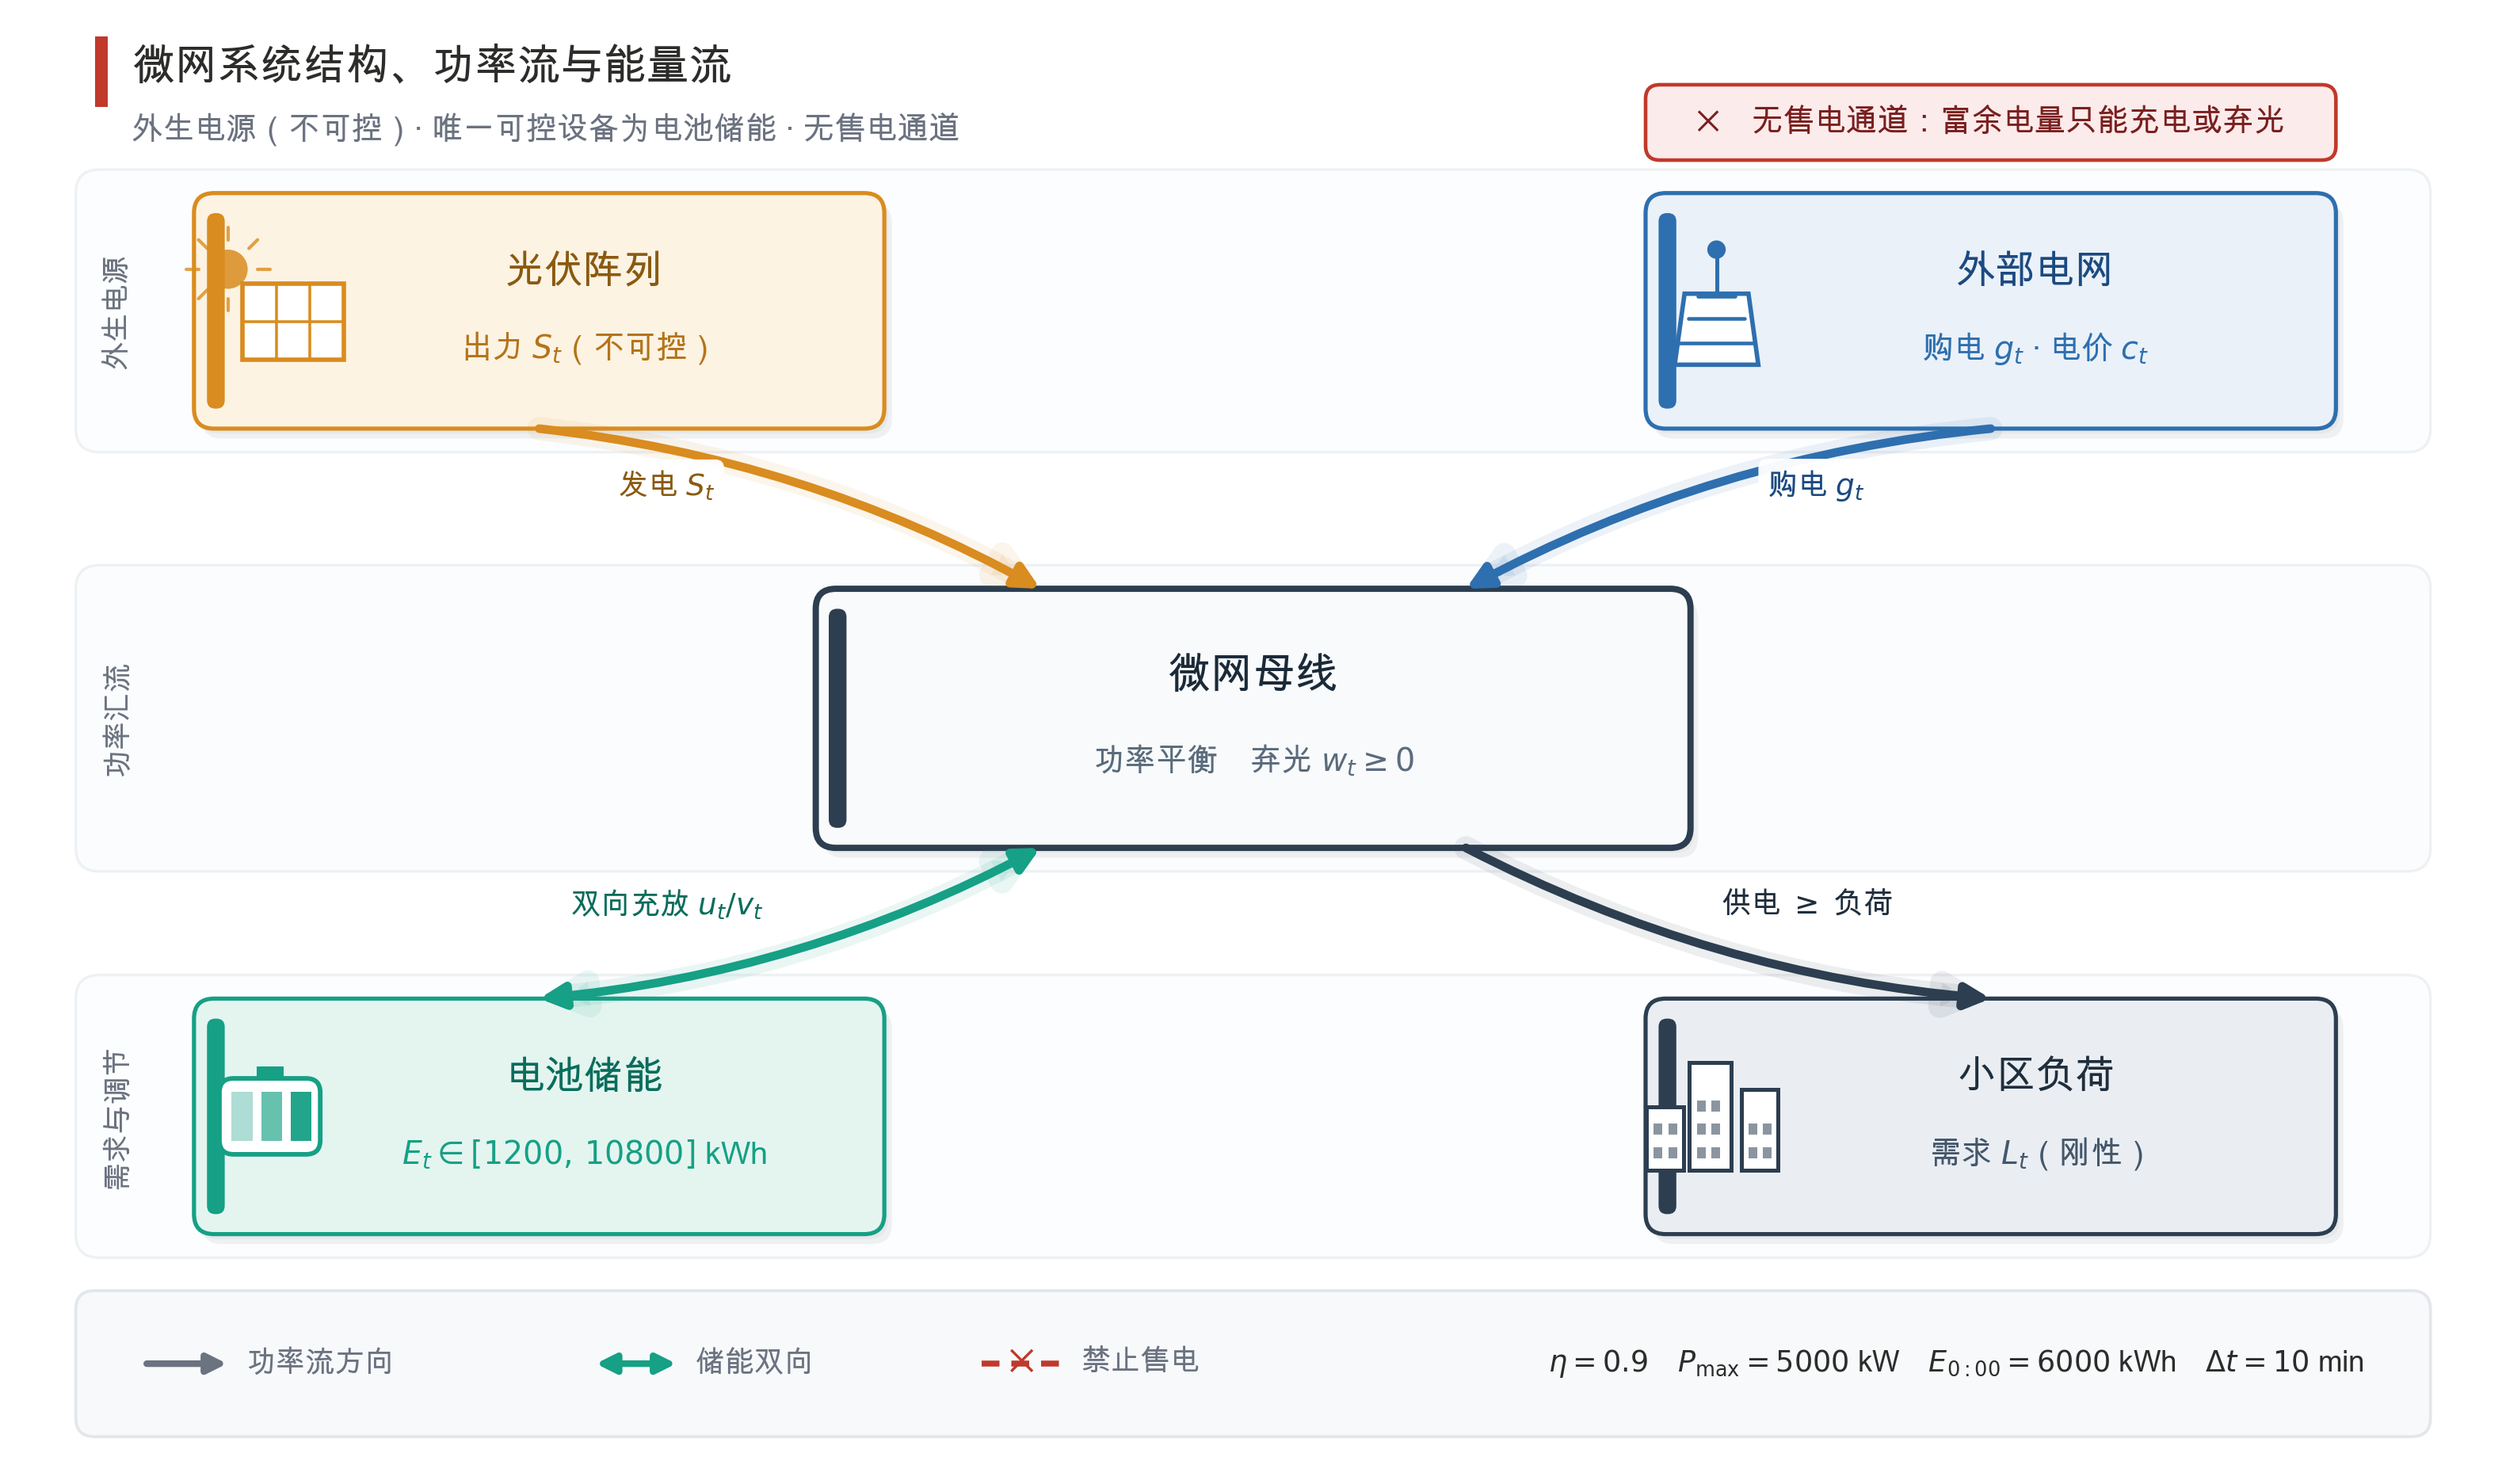
\includegraphics[width=0.9\textwidth]{fig_s1_system.png}
\caption{微电网系统结构与能量流}\label{fig:s1}
\end{figure}

\subsection{统一视角：信息集逐层收缩}
四个小问\textbf{不是四个孤立模型}，而是\textbf{同一个通用问题在四档信息集下的特例}。定义通用问题 $\mathcal{P}(\mathcal{I})$，其中 $\mathcal{I}$ 为决策时刻可获得的信息集：
\begin{align}
\min_{\{g_t,\Delta g_t,e_t,u_t,v_t,w_t,E_t\}}\ &\E\Big[\sum_{t}\big(c_t\,g_t+\gamma^{\mathrm{adj}}_t\,\Delta g_t+5c_t\,e_t\big)\Delta t\ \Big|\ \mathcal{I}\Big]\label{eq:gen}\\
\text{s.t.}\quad
& S_t+g_t+\Delta g_t+e_t+v_t=L_t+u_t+w_t, && \forall t\label{eq:genbal}\\
& E_{t+1}=E_t+\eta\Delta t\,u_t-\tfrac{\Delta t}{\eta}v_t, && \forall t\label{eq:gendyn}\\
& E_t\in[1200,10800],\ u_t,v_t\in[0,5000],\ g_t,\Delta g_t,e_t,w_t\ge 0. && \forall t
\end{align}
其中计划购电量 $g_t$ 为\textbf{承诺量}、全额按 $c_t$ 计费；$\Delta g_t$ 为调整量，罚金系数 $\gamma^{\mathrm{adj}}_t$ 依其符号取 $0.5c_t$（低于计划）或 $1.5c_t$（超出计划）；$e_t$ 为按 $5c_t$ 结算的紧急购电。四个问题即四档信息集：
\[
\I_1\supset\I_2\supset\I_3\supset\I_4,\qquad
\I_{1,2}:\ \text{电价与光伏全知},\quad
\I_3:\ \text{光伏仅有预报},\quad
\I_4:\ \text{电价亦不可预知}.
\]
$\mathcal{P}(\I_1)$、$\mathcal{P}(\I_2)$ 中随机项消失，退化为确定性 LP（问题1 单日、问题2 全年）；$\mathcal{P}(\I_3)$ 中 $S_t$ 为随机变量，本文以 MPC-II 求其\textbf{可实现策略}（问题3），并以 SDP（\S\ref{sec:sdp}）给出该档的\textbf{最优基准策略}；$\mathcal{P}(\I_4)$ 中 $c_t$ 亦进入随机项，本文以双轨法界定其费用区间（问题4）。信息越少，处理不确定性的机制必须逐层加码：由确定性 LP $\to$ 滚动重优化 $\to$ 在线决策（图~\ref{fig:s2}），全文骨架由此统一。

\begin{figure}[H]\centering
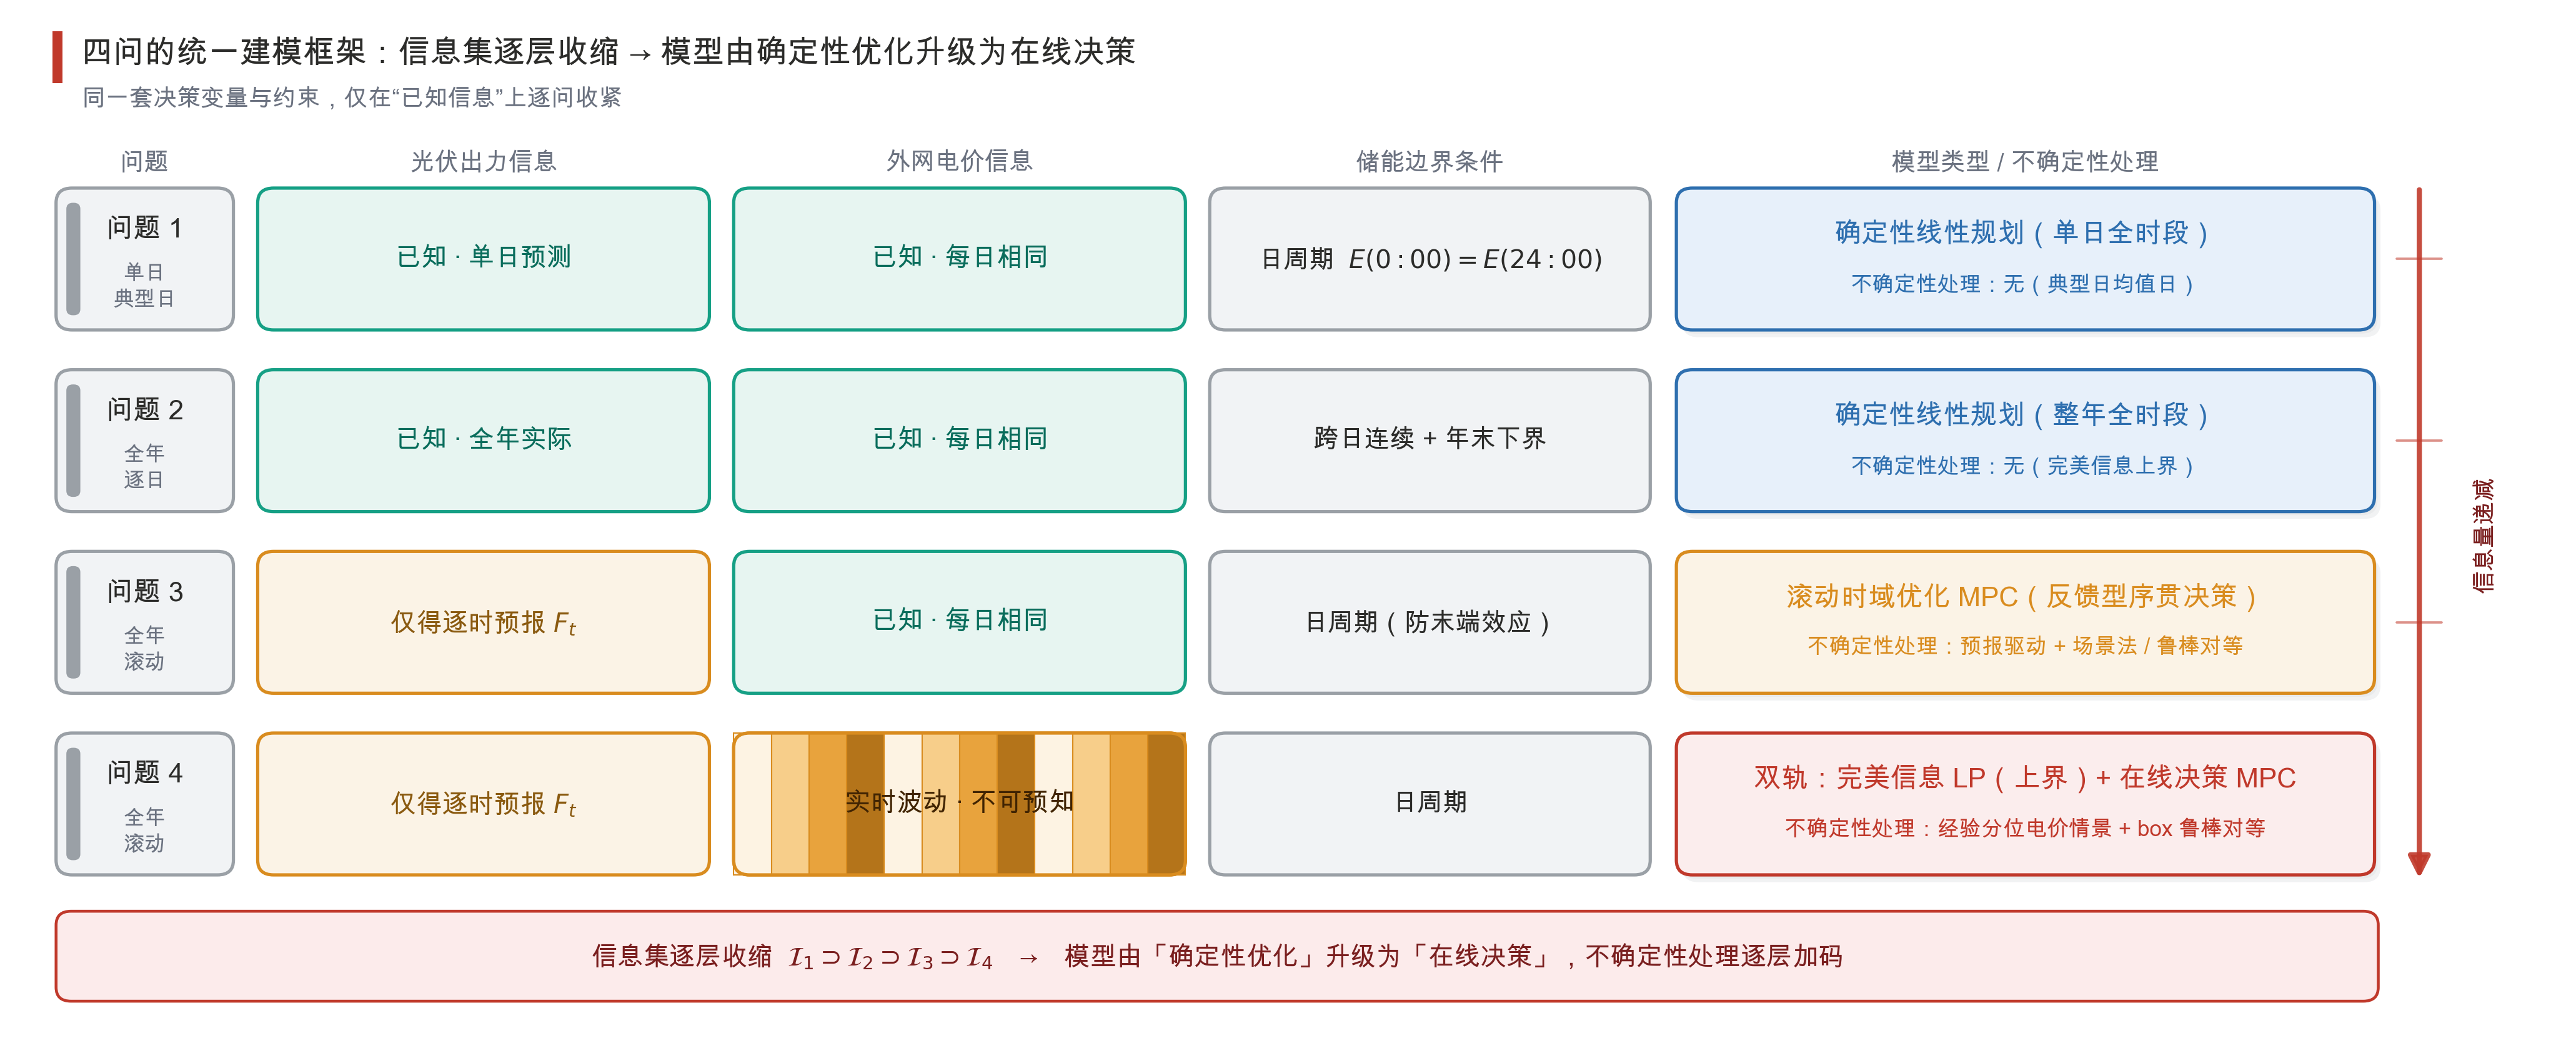
\includegraphics[width=0.98\textwidth]{fig_s2_framework.png}
\caption{四问信息集递进关系：同一模型在信息逐层收缩下的四个特例}\label{fig:s2}
\end{figure}

\subsection{技术路线：由基准到最优的递进求解}
全文的求解路线遵循\textbf{信息逐层放宽、方法逐层升级}的主线，分三步展开。

\textbf{步骤一：确定性基准（问题1--2）}。光伏与电价全知，通用问题 \eqref{eq:gen} 中的随机项消失，直接以确定性 LP 精确求解：问题1 建立单日模板并作对偶分析，问题2 放大到全年；同时保留\textbf{完美信息 + 日周期}方案，作为后续一切不确定性模型的对照下界。

\textbf{步骤二：滚动修正（问题3）}。光伏只剩预报。先以\textbf{最朴素的滚动优化}为基线；继而由题面的 take-or-pay 条款（计划量全额计费 + 偏离罚金 + 5 倍紧急购电）推出\textbf{调整环节的边际成本是罚金而非购电成本}，据此将基线修正为\textbf{罚金感知的滚动时域优化（MPC-II）}。修正之后自然产生一问：\textbf{所提策略距离同信息结构下的最优还有多远？}

\textbf{步骤三：最优性基准（\S\ref{sec:sdp}）}。以随机动态规划（SDP）解出全体策略，为步骤二之问给出定量回答：MPC-II 的费用与 SDP 最优策略仅差 0.16\%，并分离出\textbf{决策方法}与\textbf{预报精度}两类改进空间（2.66\% vs 13.45\%）。

\textbf{问题4} 将电价维度纳入同一框架：把\textbf{电价已知}与\textbf{电价不可预知}两轨并列，其差即电价不确定性的精确价格，再辅以经验分位情景与 $\Gamma$ 型鲁棒对等，形成\textbf{期望--最坏}双视角。

\section{模型假设与符号说明}

\subsection{模型假设}
\begin{enumerate}[label=\textbf{A\arabic*.}]
  \item 各时段内功率恒定，10 分钟电量 = 功率 $\times\Delta t$，$\Delta t=1/6$ h；
  \item 储能充放电效率各为 $\eta=0.9$（题目给\textbf{效率 90\%}，取双侧各 90\%，并在灵敏度中对 $\eta$ 做扫描）；储能无自放电；容量限制 $E\in[1200,10800]$ kWh、功率 $|u|,|v|\le 5000$ kW；
  \item \textbf{不允许向电网售电}：多余电量必须弃光（题面无售电通道）；
  \item 问题1--2 中附件数据视为完美信息；问题3 中计划基于预报制定，实际光伏按附件2 结算，短缺触发紧急购电、盈余弃光；
  \item \textbf{口径A（主口径）}：计划购电量全额按交易电价计费（题面原文\textbf{除紧急购电费用外，其他时间段的购电费用均按计划购电量计算}），调整环节的偏离按 0.5/1.5 倍罚金计费；
  \item 问题3/4 交付期为 2025-02-01 至 12-31（334 天），1 月作为储能由初值滚动至稳态的预热期；
  \item 预报数据的 10 分钟粒度值由整点预报经 PCHIP 保形插值降尺度获得，发布时刻本身的锚点值采用\textbf{当日更早一次预报对该时刻的预测}，保证决策只用当时可得信息。
\end{enumerate}

\subsection{符号说明}
\begin{table}[H]\centering\small
\caption{主要符号}\label{tab:sym}
\begin{tabular}{ll@{\qquad}ll}
\toprule
符号 & 含义 & 符号 & 含义\\
\midrule
$c_t$ & 时段 $t$ 电价（元/kWh） & $L_t,\hat S_t,S_t$ & 负载、预报光伏、实际光伏 (kW)\\
$g_t$ & 购电功率（kW） & $u_t,v_t$ & 充、放电功率（kW）\\
$w_t$ & 弃光功率（kW） & $E_t$ & 时段末储电量（kWh）\\
$\eta$ & 充/放电效率 & $g^0_t$ & 0:00 制定的计划购电量\\
$a_t$ & 调整购电量（执行量） & $d^{+}_t,d^{-}_t$ & 调整超出/不足计划的部分\\
$\sigma(k)$ & 提前期 $k$ 小时的预报误差标准差 & $\Gamma$ & 鲁棒预算系数\\
\bottomrule
\end{tabular}
\end{table}

\section{数据探索与预报误差标定}

\subsection{附件1 是\textbf{全年平均日}}
实测验证：附件1 的电价曲线与附件4 全年逐时段均值之最大偏差 $5.15\times10^{-5}$，负载、光伏同样吻合（差异均在四舍五入量级）。故附件1 并非随意给出的一天，而是\textbf{典型日基准场景}；问题2 相对\textbf{问题1 方案外推}的费用差包含两块——逐日精细化的真实价值与 Jensen 缺口（\S\ref{sec:jensen}）。

\subsection{预报误差的标定：离散度主导}
将附件3 各发布时刻的预报与附件2 实际逐时对齐（白天样本），统计 $\varepsilon_k=\hat S_k-S$：
\[
\sigma(k):\ 57.9\to1257.3\ \text{kW}\ (\times 21.7),\quad
\mathrm{MAE}(k):\ 37.4\to750.1\ \text{kW},\quad
\bar\varepsilon:\ +2.4\to-208.6\ \text{kW}.
\]
三点结论：① 误差离散度随提前期近似幂律放大（$\sigma(k)\approx 58\,k^{0.97}$）；② 均值偏差很小且方向为\textbf{预报偏低（保守）}，全年电量口径预报 20\,015 MWh vs 实际 20\,251 MWh（低估 1.2\%），$|\bar\varepsilon_{24}|/\sigma_{24}\approx0.17$；③ 误差分布左偏、异方差。因此\textbf{紧急购电风险由离散度而非均值偏差驱动}，建模重点是 $\sigma(k)$ 与经验分位形态，而非常数偏差修正（图~\ref{fig:calib}）。

\begin{figure}[H]\centering
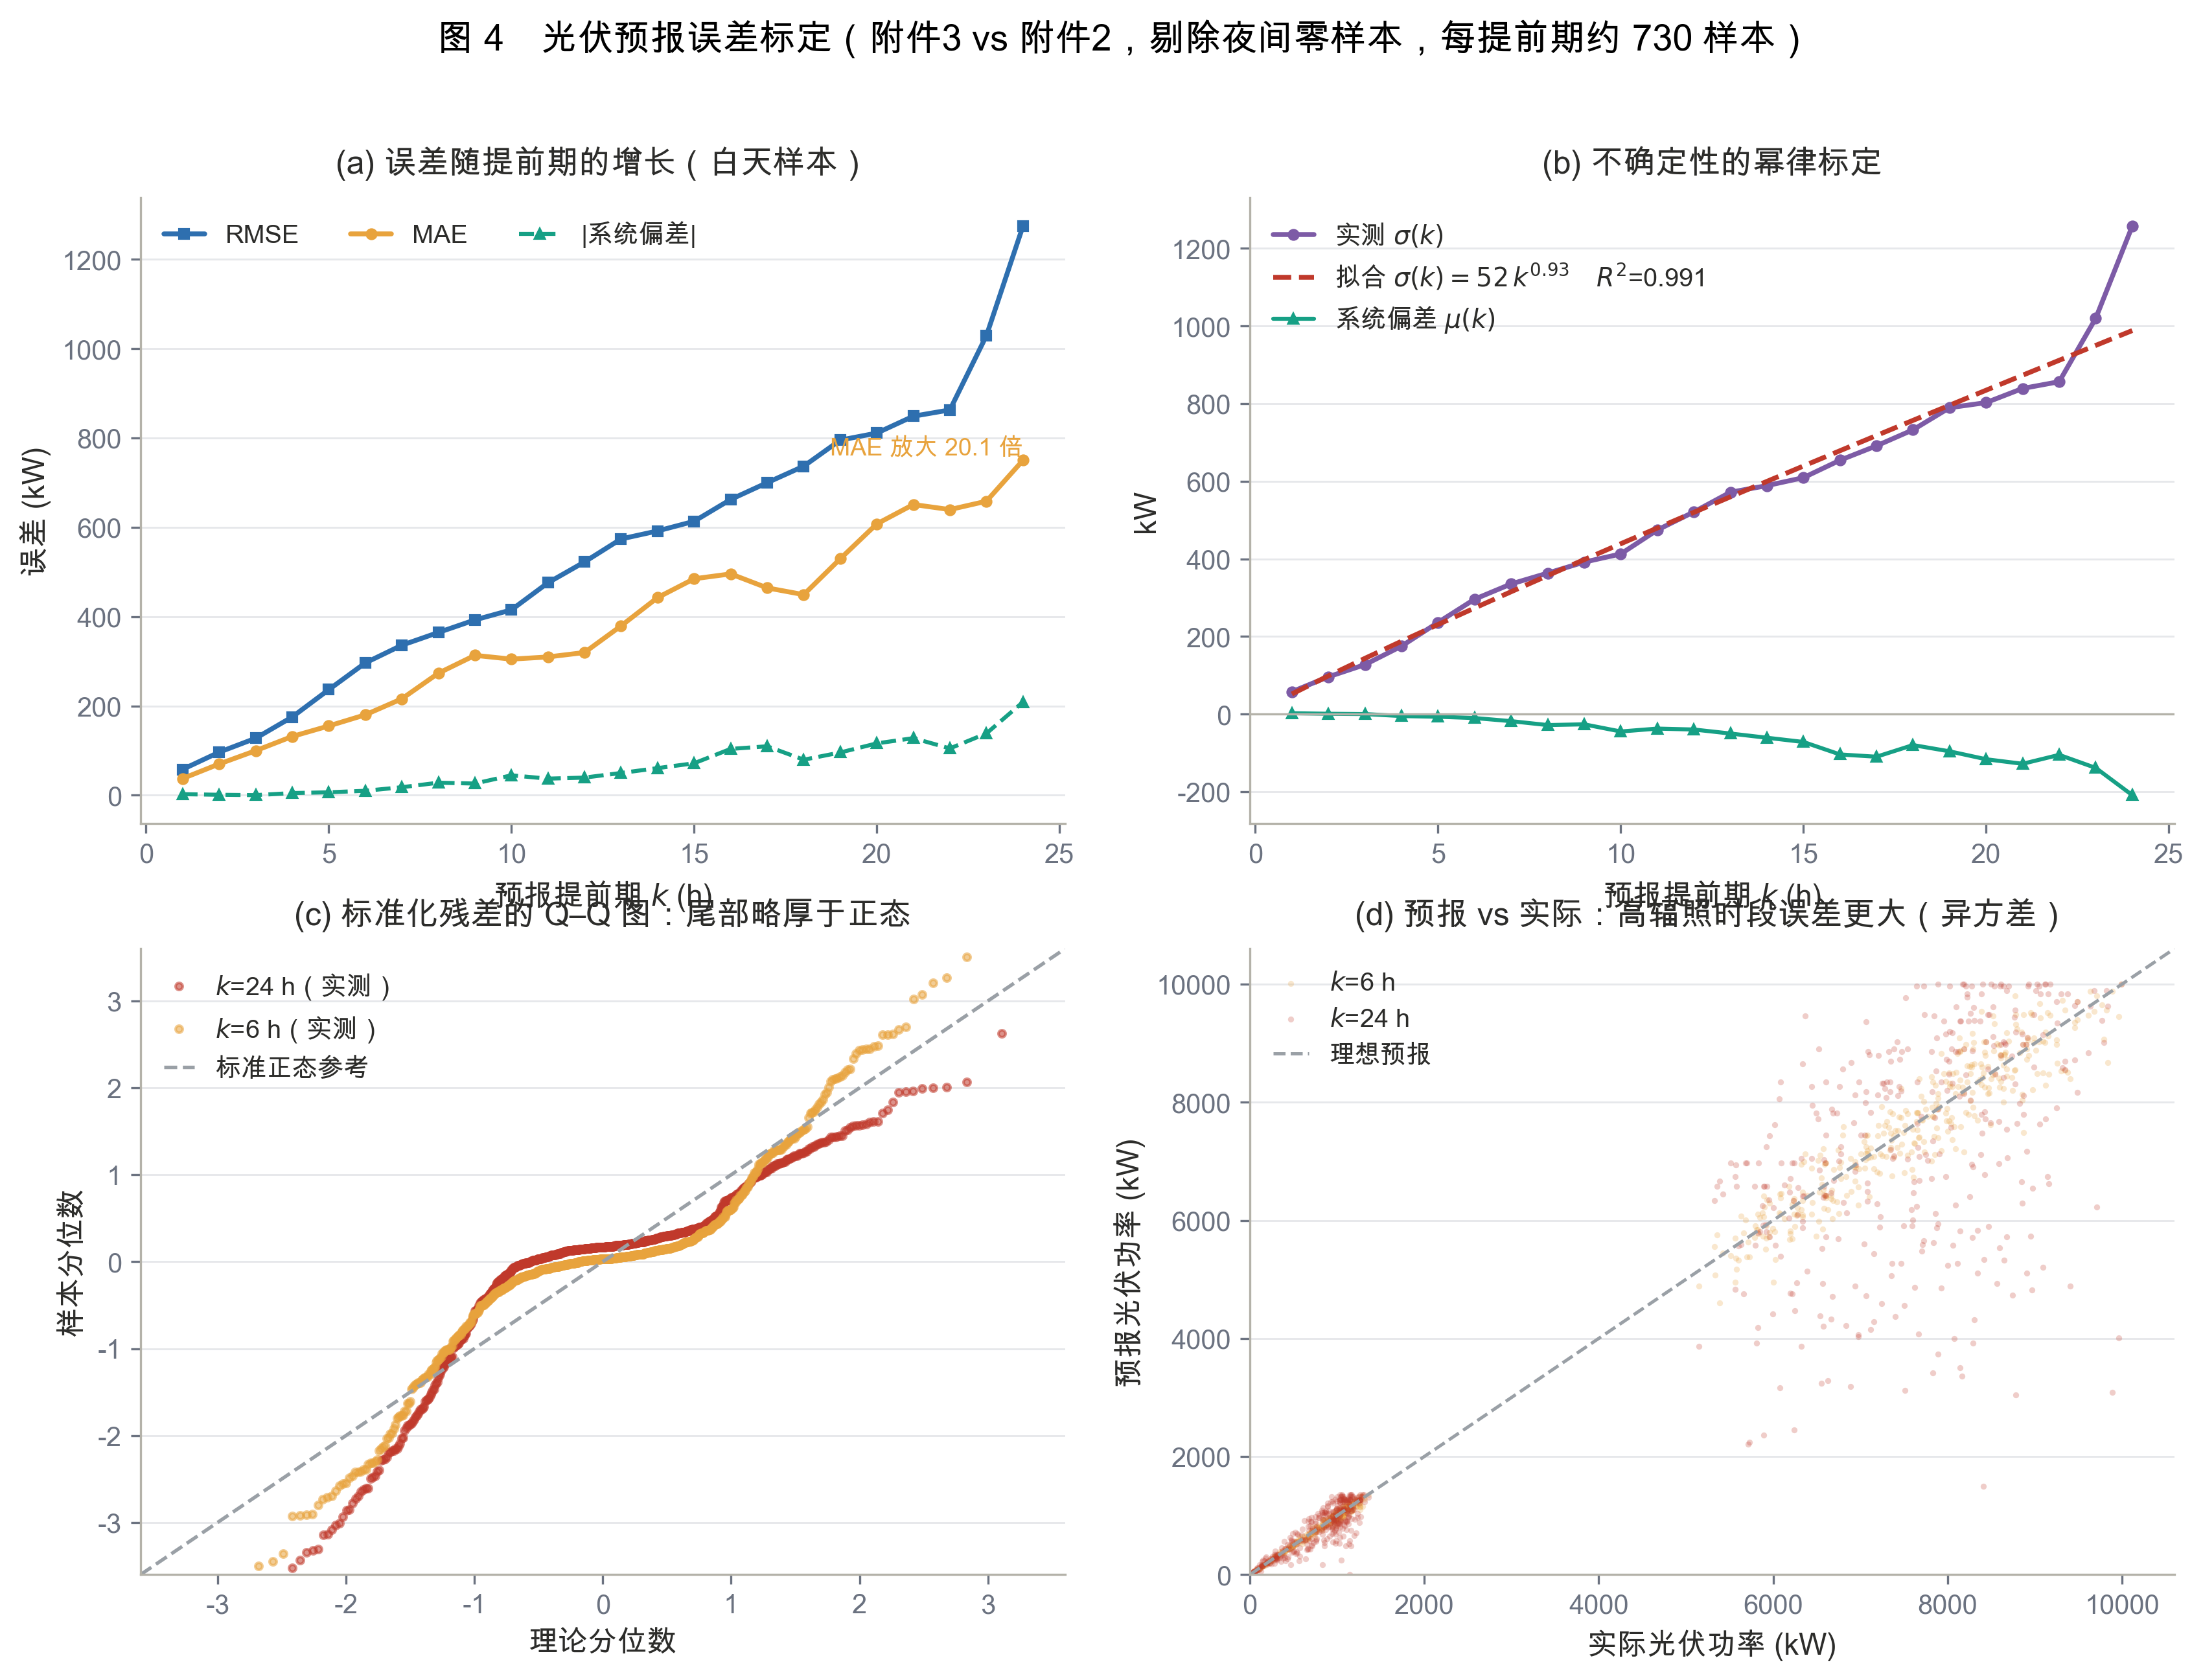
\includegraphics[width=0.98\textwidth]{fig_p3_forecast_calib.png}
\caption{光伏预报误差标定：误差随提前期放大（左上）、偏差量级远小于离散度（右上）、标准化残差近似正态（左下）、$\sigma(k)$ 幂律拟合（右下）}\label{fig:calib}
\end{figure}

\section{问题1：单日确定性线性规划与对偶分析}\label{sec:p1}

\subsection{模型}
决策变量为各时段购电、充、放电与弃光功率 $g_t,u_t,v_t,w_t\ (t=1,\dots,144)$ 及储电量 $E_t$：
\begin{align}
\min\ & \sum_{t=1}^{144} c_t\,g_t\,\Delta t \label{eq:p1obj}\\
\text{s.t.}\quad
& g_t+v_t+\hat S_t=L_t+u_t+w_t, && \forall t \quad(\text{功率平衡})\label{eq:p1bal}\\
& E_t=E_{t-1}+\eta\Delta t\,u_t-\tfrac{\Delta t}{\eta}v_t,\ E_0=6000, && \forall t \quad(\text{储能动态})\label{eq:p1dyn}\\
& 1200\le E_t\le10800,\ 0\le u_t,v_t,w_t\le5000,\ g_t\ge0,\ && \forall t\\
& E_{144}=E_0. && (\text{日周期})\label{eq:p1cyc}
\end{align}
注意 \eqref{eq:p1bal} 中放电 $v_t$ 受净负荷约束 $v_t\le\max(L_t-\hat S_t,0)$ 的隐式限制（不许售电由平衡式与 $w_t\ge0$ 共同保证：放电超出净负荷必然产生 $w_t>0$ 且不经济，最优解自动排除）。

\subsection{求解结果}
HiGHS 直接求解：\textbf{全天购电量 59\,482.699 kWh，购电费 35\,126.949 元}。校验：理论下界（无储能净负荷电量）56\,729 kWh，最优解高于下界 4.9\%，全部来自往返效率损耗，无凭空造电；储能净变化与终端约束恒等式残差 $<10^{-9}$。调度形态呈典型\textbf{双峰套利}：低谷（22:00 后，0.58 元）充满，早高峰放电，午间以光伏余电 + 低价谷电二次充电，晚高峰最高价 1.3952 元时刻恰好放空（图~\ref{fig:p1}）。

\begin{figure}[H]\centering
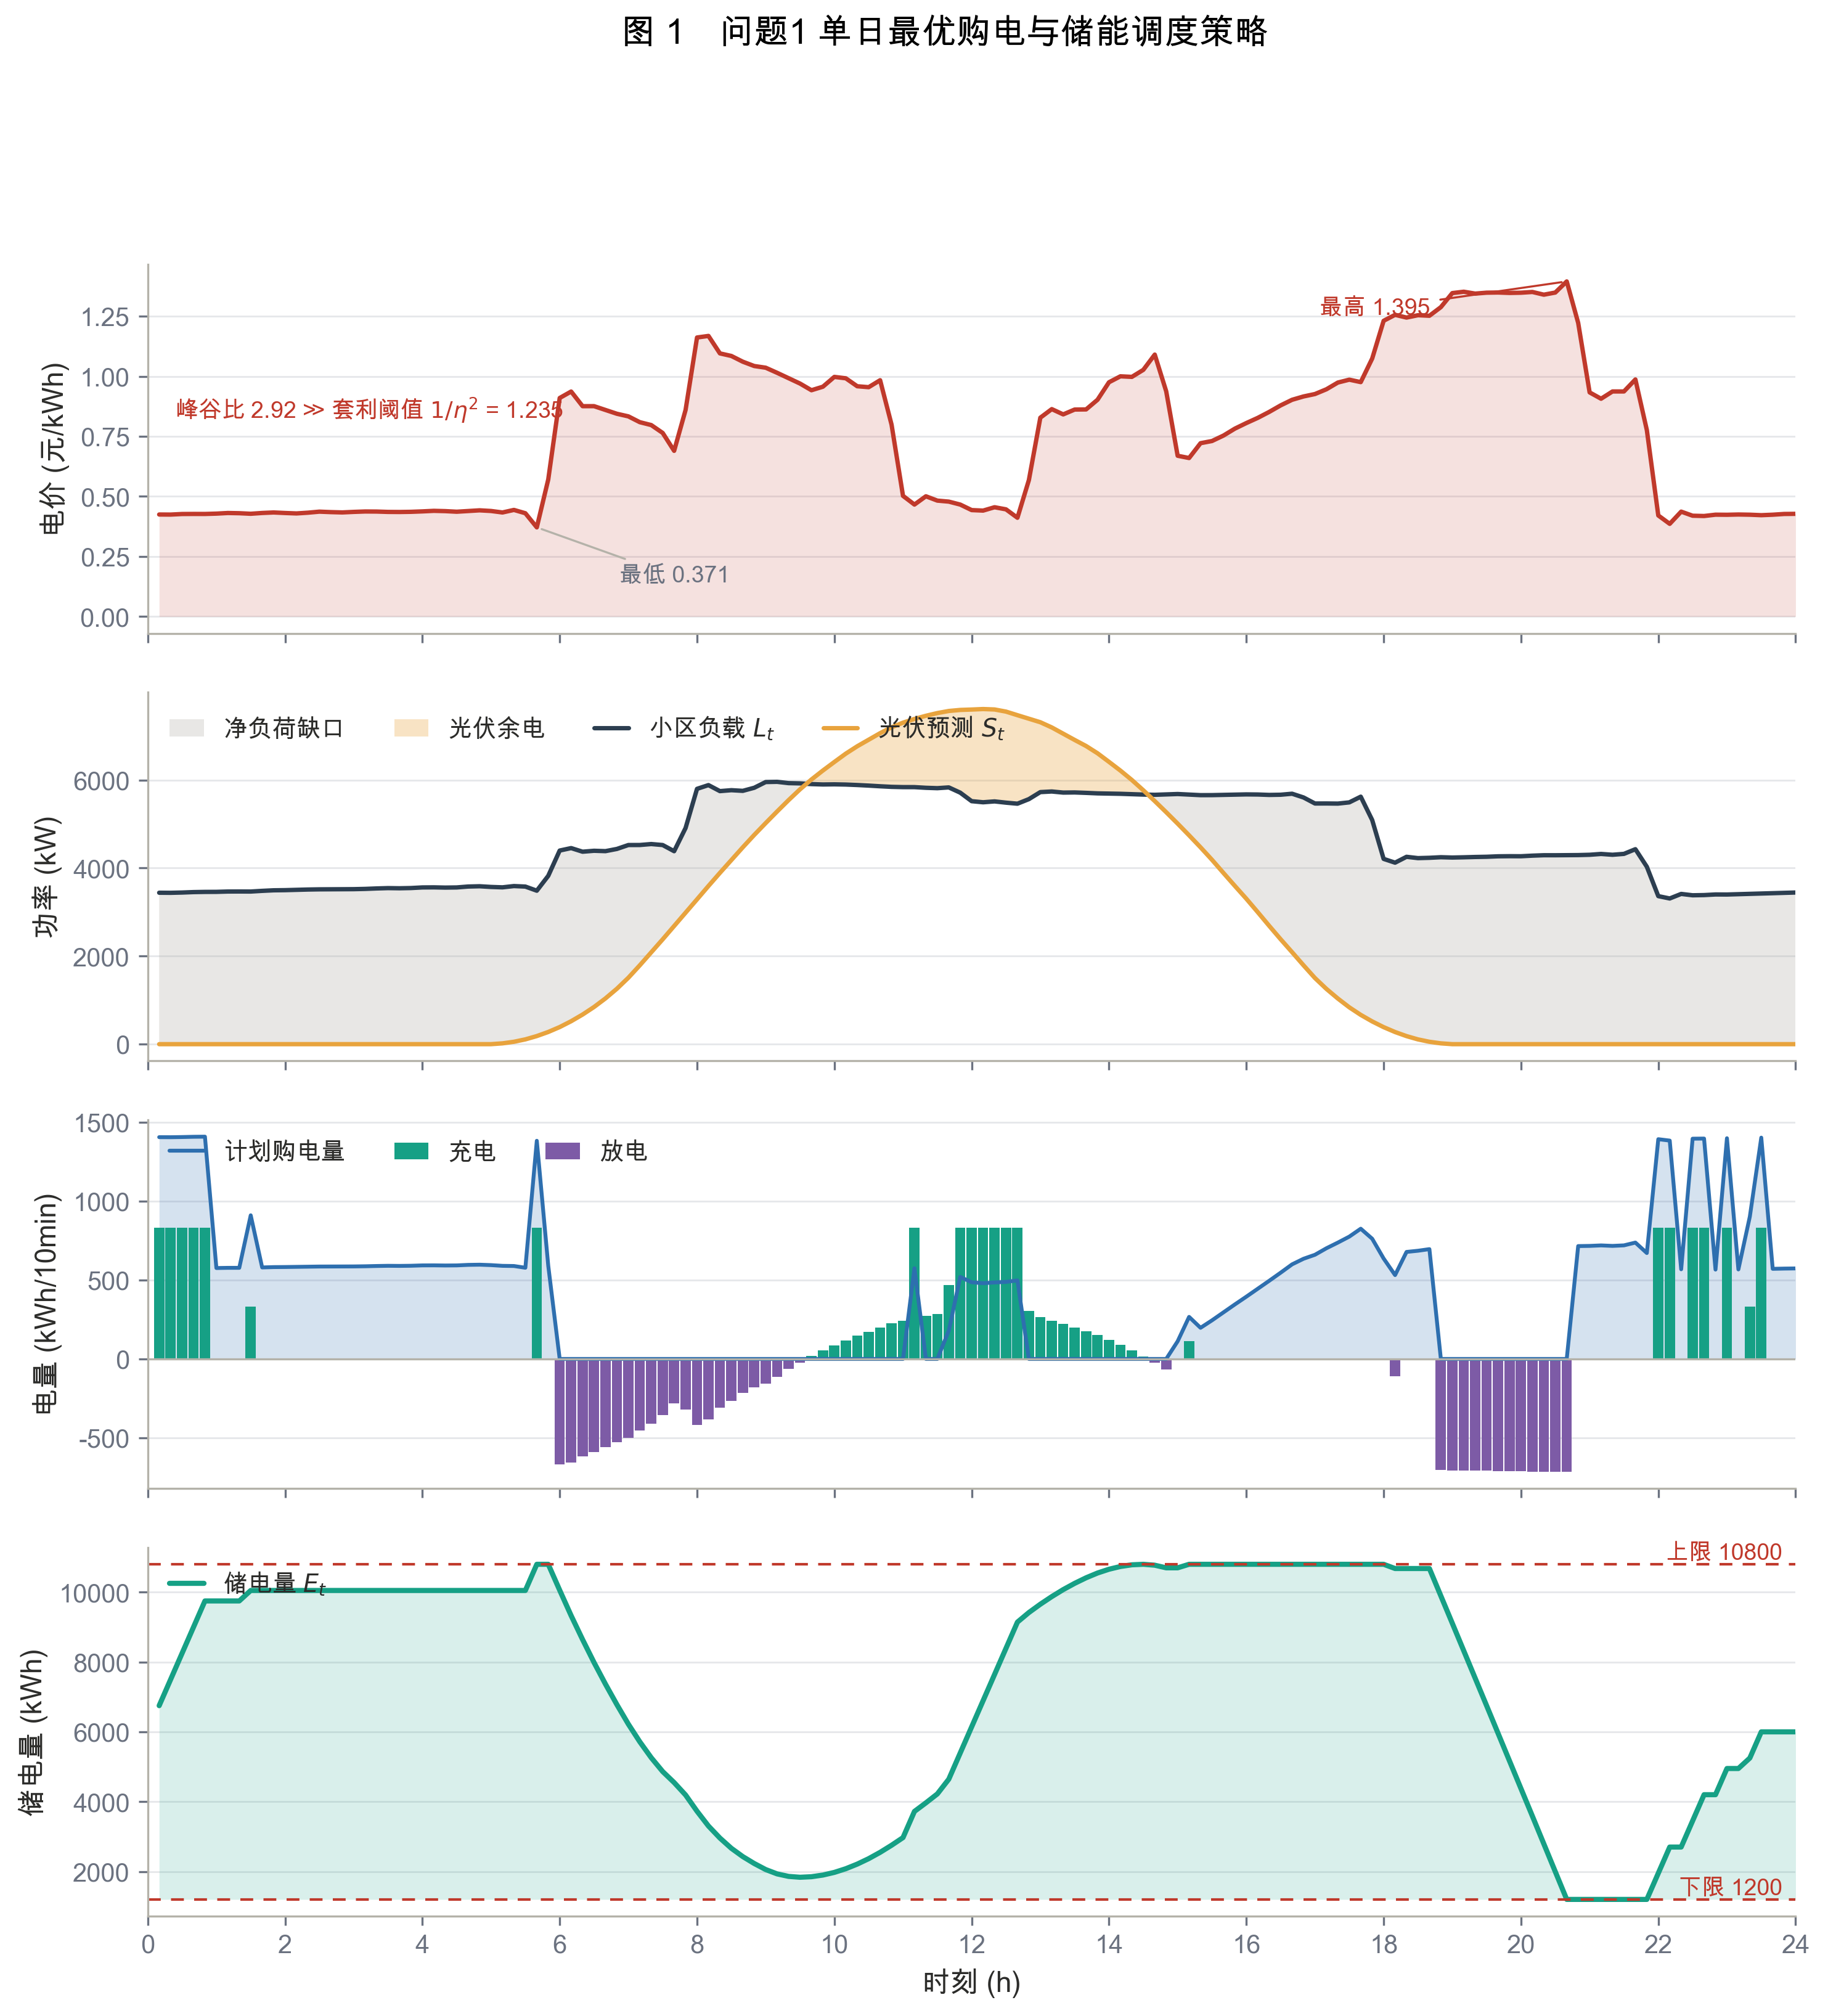
\includegraphics[width=0.98\textwidth]{fig_p1_dispatch.png}
\caption{问题1 典型日调度方案：(a) 电价与套利区间；(b) 净负荷与光伏；(c) 储能充放电与储电量轨迹；(d) 分时购电量}\label{fig:p1}
\end{figure}

\subsection{对偶分析：套利阈值与边际电源排序}
LP 对偶变量给出边际价格 $\mu_t$。互补松弛条件数值验证：购电时段 $\mu_t=c_t$（残差 $1.1\times10^{-16}$），非购电时段 $\mu_t<c_t$。由储能动态约束的对偶可推出\textbf{套利判据}：峰谷比超过 $1/\eta^2=1.235$ 时储能往返套利才有利可图；实测平均日峰谷比 2.92，全年日内峰谷比中位数 4.331 且 \textbf{365/365 天全部越线}——每一天都值得套利（图~\ref{fig:p1dual}）。

\begin{figure}[H]\centering
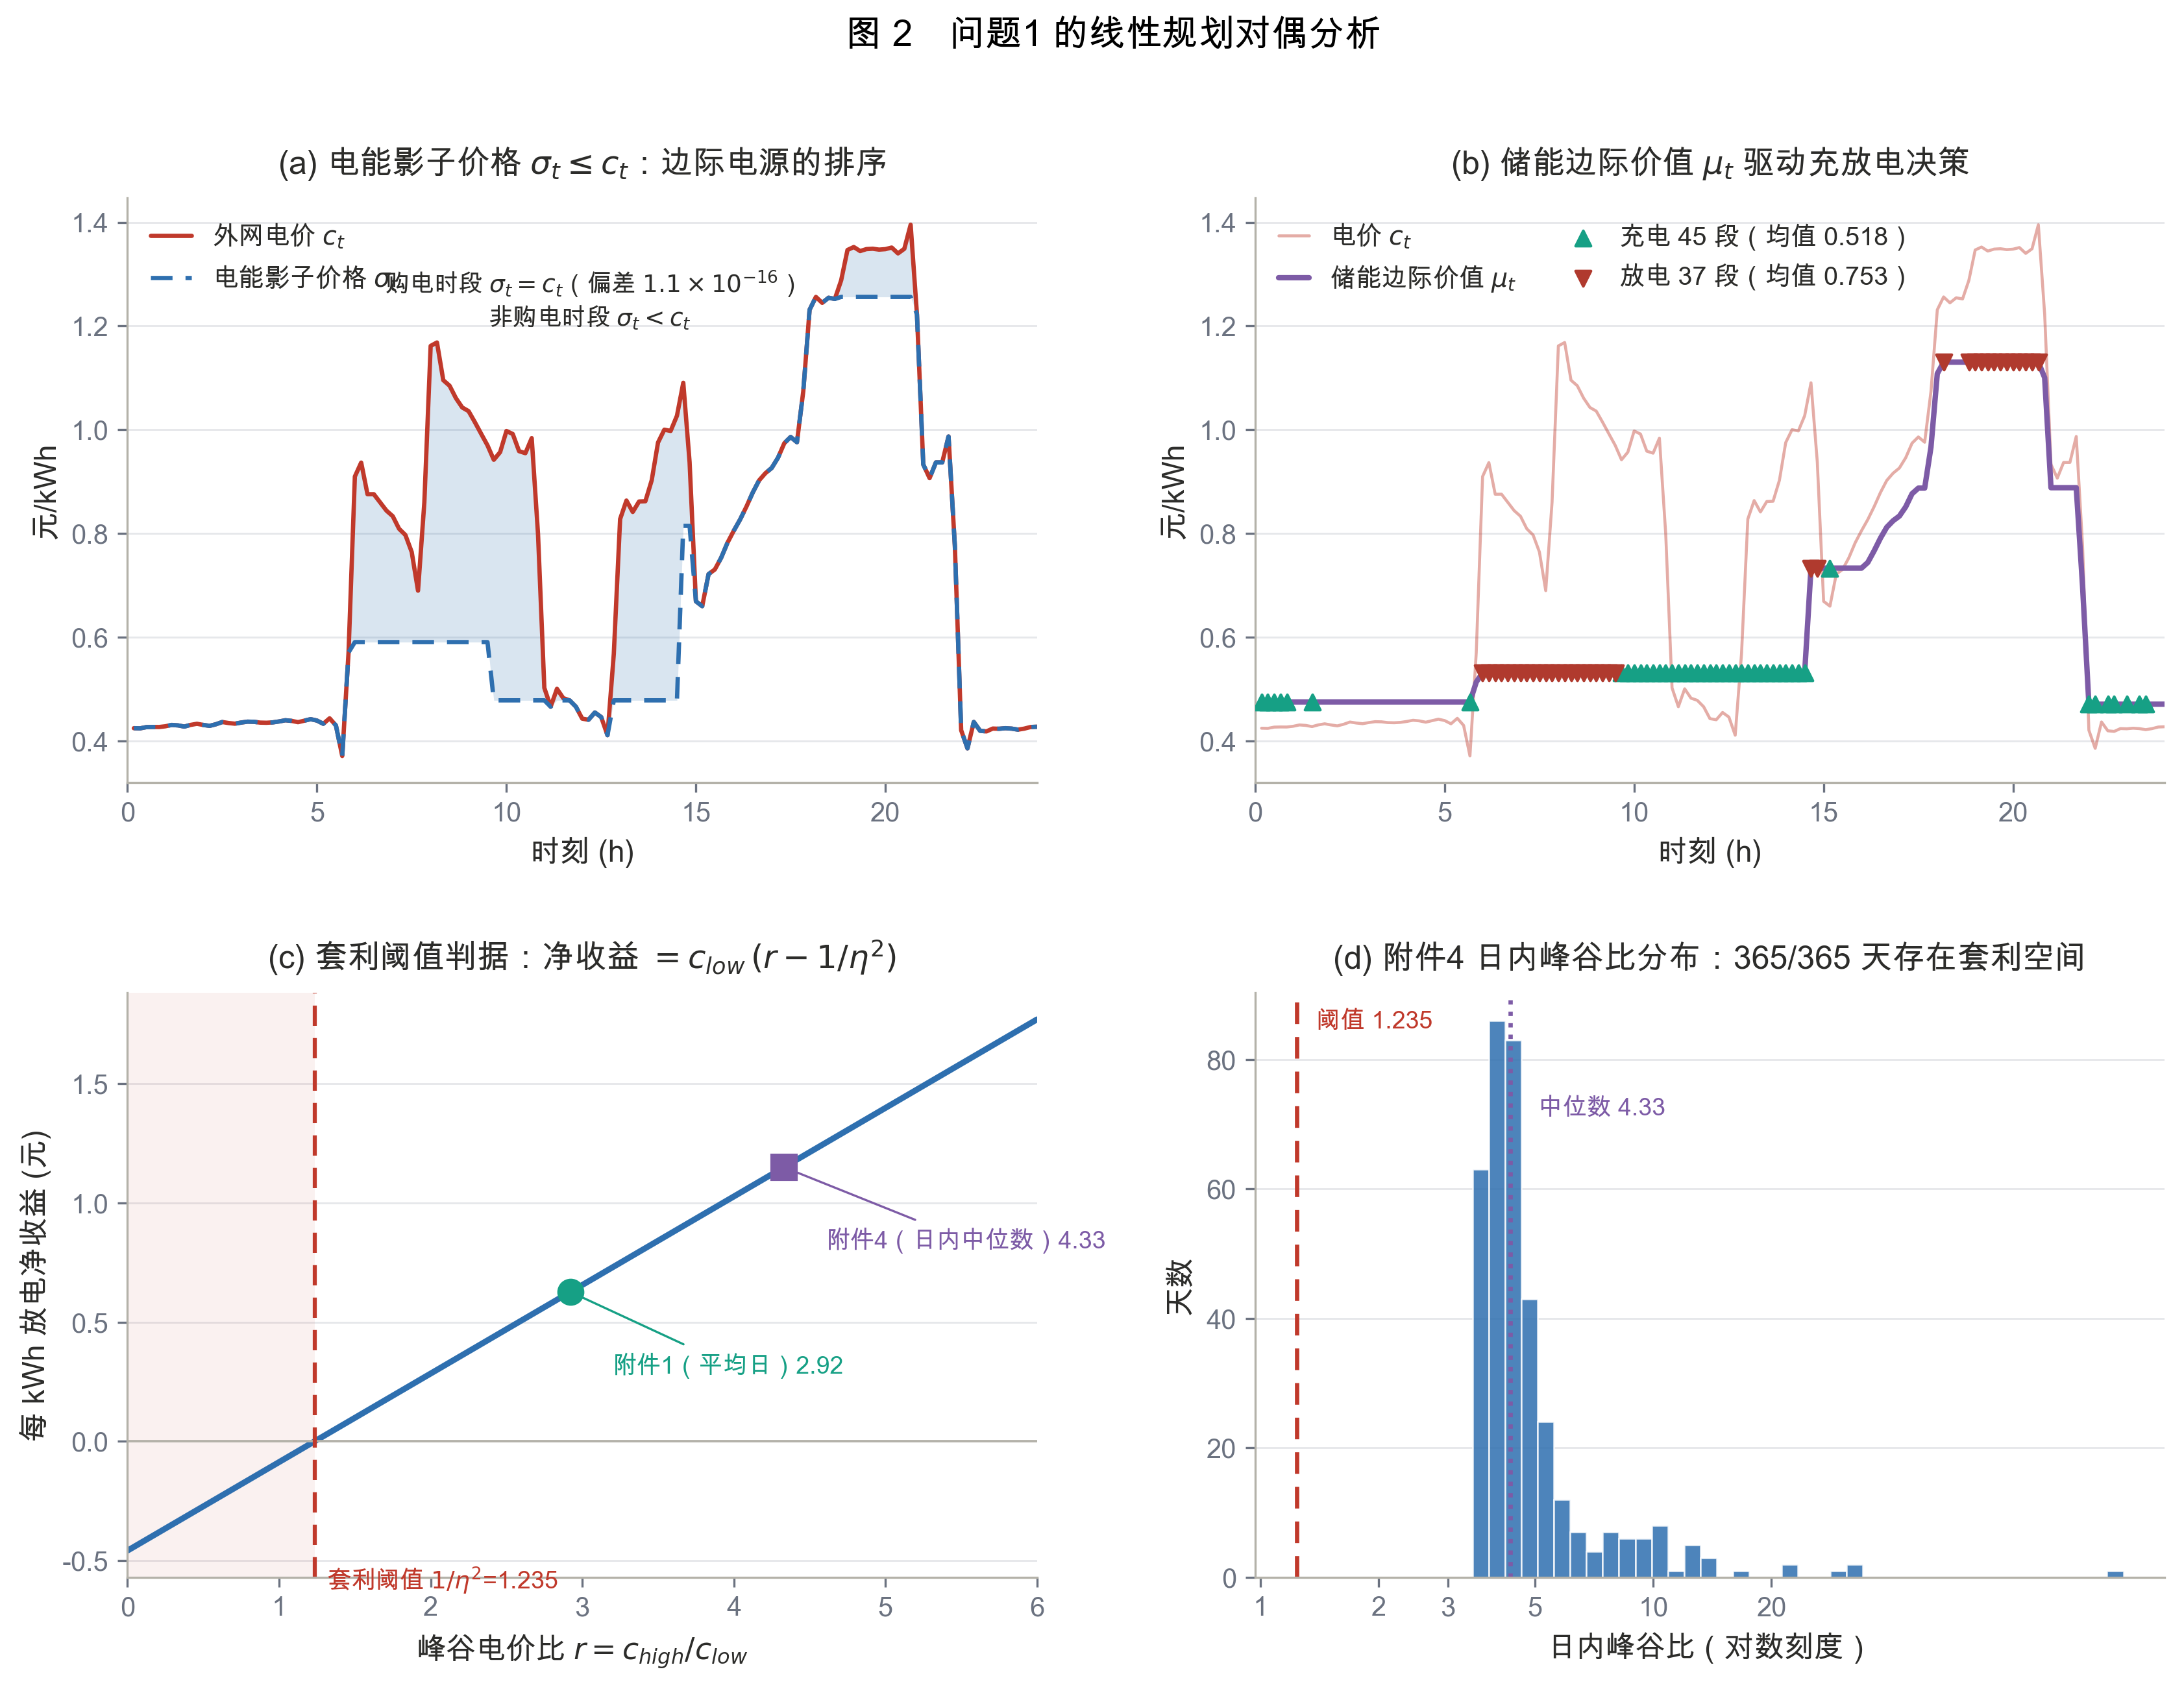
\includegraphics[width=0.98\textwidth]{fig_p1_dual.png}
\caption{问题1 对偶分析：影子价格与电价的互补松弛（左）与储能在边际电价排序中的位置（右）}\label{fig:p1dual}
\end{figure}

题面要求的结果见表~\ref{tab:p1t1}、表~\ref{tab:p1t2}（数值由求解结果直接导出）。

% ================= 问题1 表1/表2
\begin{table}[H]\centering\small
\caption{问题1：微网在指定时间段的购电量及全天购电量和购电费}\label{tab:p1t1}
\begin{tabular}{lrr}
\toprule
项目 & 数值 & 单位\\
\midrule
10:00-10:10 & 0.000 & kWh\\
12:00-12:10 & 486.403 & kWh\\
14:00-14:10 & 0.000 & kWh\\
16:00-16:10 & 394.931 & kWh\\
18:00-18:10 & 636.983 & kWh\\
20:00-20:10 & 0.000 & kWh\\
\midrule
全天购电量 & 59,482.699 & kWh\\
全天购电费 & 35,126.949 & 元\\
\bottomrule\end{tabular}\end{table}
\begin{table}[H]\centering\small
\caption{问题1：储能设备在指定时间段的充放电量及储电量}\label{tab:p1t2}
\begin{tabular}{lrr}
\toprule
时间段 & 充电量 (kWh) & 放电量 (kWh)\\
\midrule
00:00-04:00 & 4,500.0 & 0.0\\
04:00-08:00 & 833.3 & 6,365.8\\
08:00-12:00 & 4,788.0 & 1,703.0\\
12:00-16:00 & 5,286.0 & 91.1\\
16:00-20:00 & 0.0 & 5,780.1\\
20:00-24:00 & 5,333.3 & 2,859.9\\
\midrule
0:00 储电量 & \multicolumn{2}{c}{6,000 kWh}\\
24:00 储电量 & \multicolumn{2}{c}{6,000.0 kWh}\\
\bottomrule\end{tabular}\end{table}

\section{问题2：全年连续线性规划}\label{sec:p2}

\subsection{模型}
将 \eqref{eq:p1obj}--\eqref{eq:p1dyn} 沿时间轴拼接：全年 $52\,560$ 个时段，决策变量 $262\,800$ 个，等式约束 $105\,121$ 个；日周期约束 \eqref{eq:p1cyc} 放宽为年末约束 $E_{\text{末}}\ge E_0$（更弱、更贴近题意）。电价采用附件4 波动序列 $c_t$，负载与光伏采用附件2 实际值。

\subsection{求解结果}
HiGHS \textbf{3 秒}求解完毕（稀疏 COO 装配 + 双精度）。全年购电费 \textbf{12\,229\,460.73 元}：
\begin{itemize}
  \item 无储能基线（净负荷直接购电）16\,407\,319.63 元，储能套利\textbf{节省 25.5\%}；
  \item \textbf{完美信息 + 日周期}口径（与问题1 同构，作为问题3 的对照基线）12\,245\,046.92 元；
  \item 问题1 平均日方案外推 334 天仅 11\,732\,401.30 元，比真实逐日最优\textbf{低估 9.32\%}——见下。
\end{itemize}

\subsection{Jensen 缺口：平均日模型必然低估}\label{sec:jensen}
购电费对负荷/光伏剖面是\textbf{凸函数}，平均剖面抹平了日内与逐日波动，故 $\E[c\,g^*(L,S)]\ge c\,g^*(\E[L,S])$。实测：问题1 日均购电费 35\,127 元 vs 问题2 真实日均 37\,681 元（差 7.27\%），全年低估 932\,147 元。这不是模型错误，而是\textbf{确定性典型日方法的结构性偏差}，也定量说明了逐日精细化的价值上限。

图~\ref{fig:p2} 给出全年策略全景，图~\ref{fig:p2dual} 从对偶视角解释机制：光伏渗透率越高的月份储能边际价值越低（$r=-0.995$）；弃光由\textbf{储能饱和且光伏富余}触发。题面要求的指定日期结果见表~\ref{tab:p2t1}、表~\ref{tab:p2t2}。

\begin{figure}[H]\centering
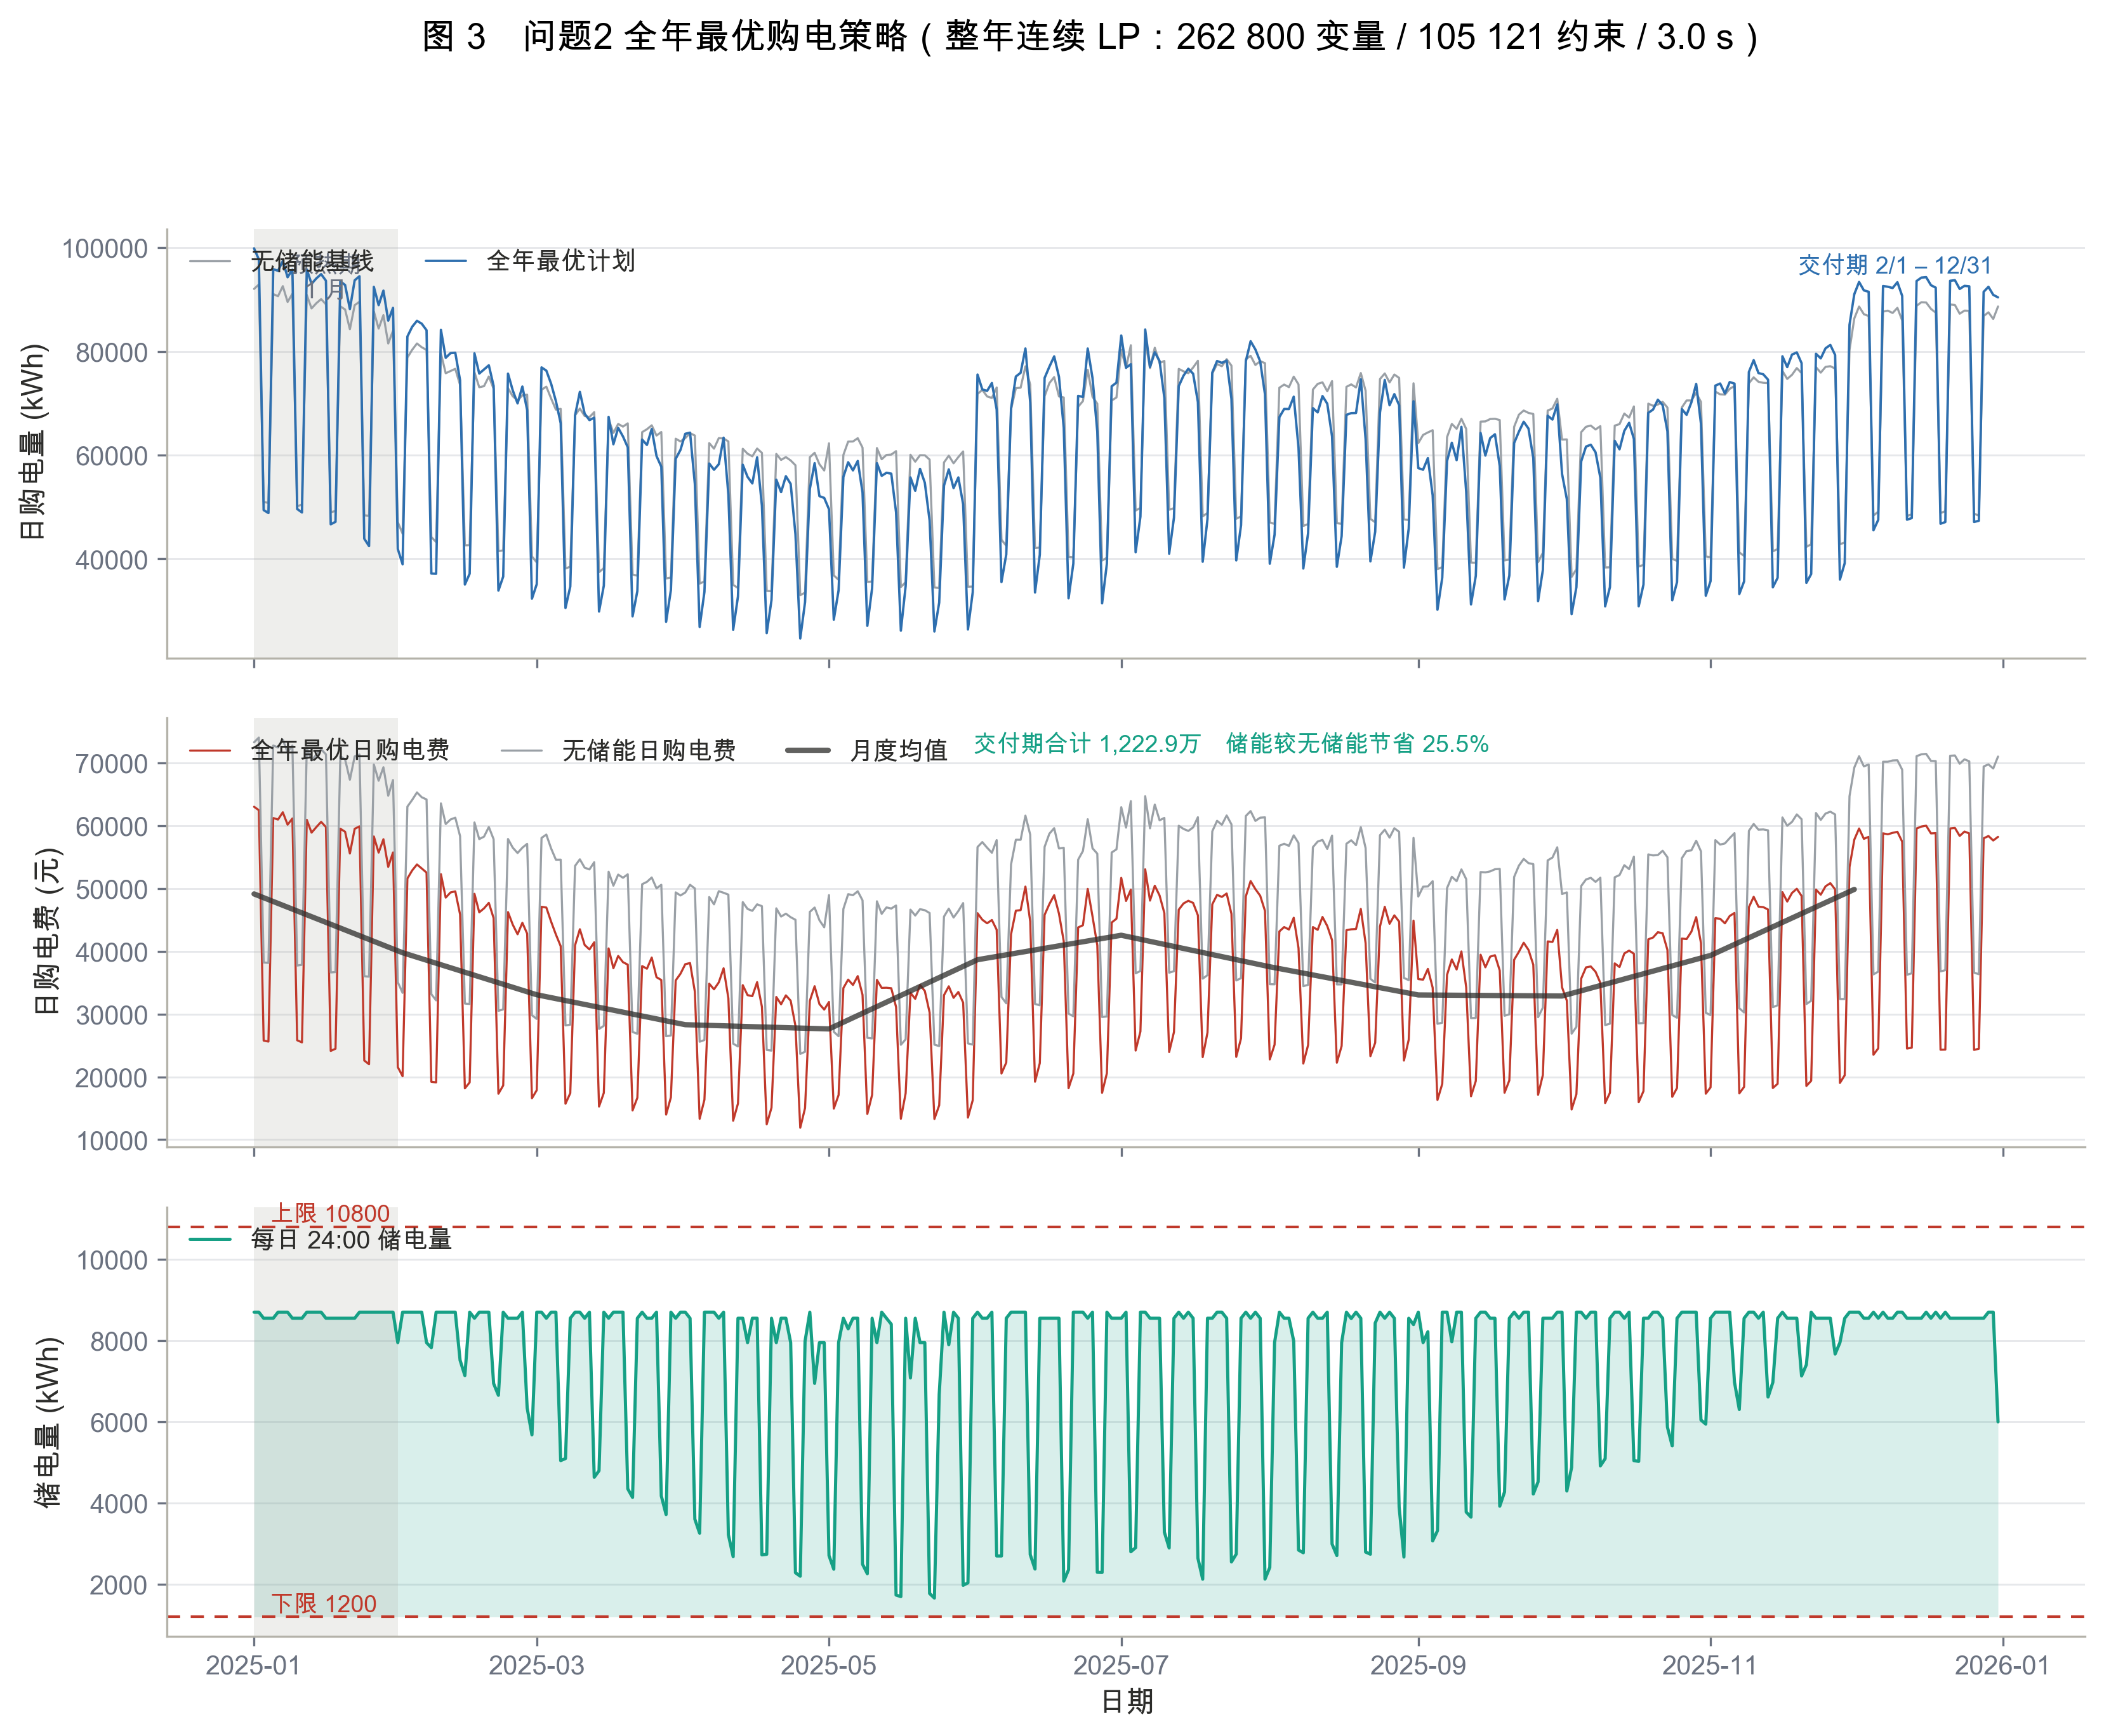
\includegraphics[width=0.98\textwidth]{fig_p2_year.png}
\caption{问题2 全年策略：(a) 月度购电费；(b) 储能动作与储电量；(c) 弃光分布；(d) 峰谷比分布}\label{fig:p2}
\end{figure}

\begin{figure}[H]\centering
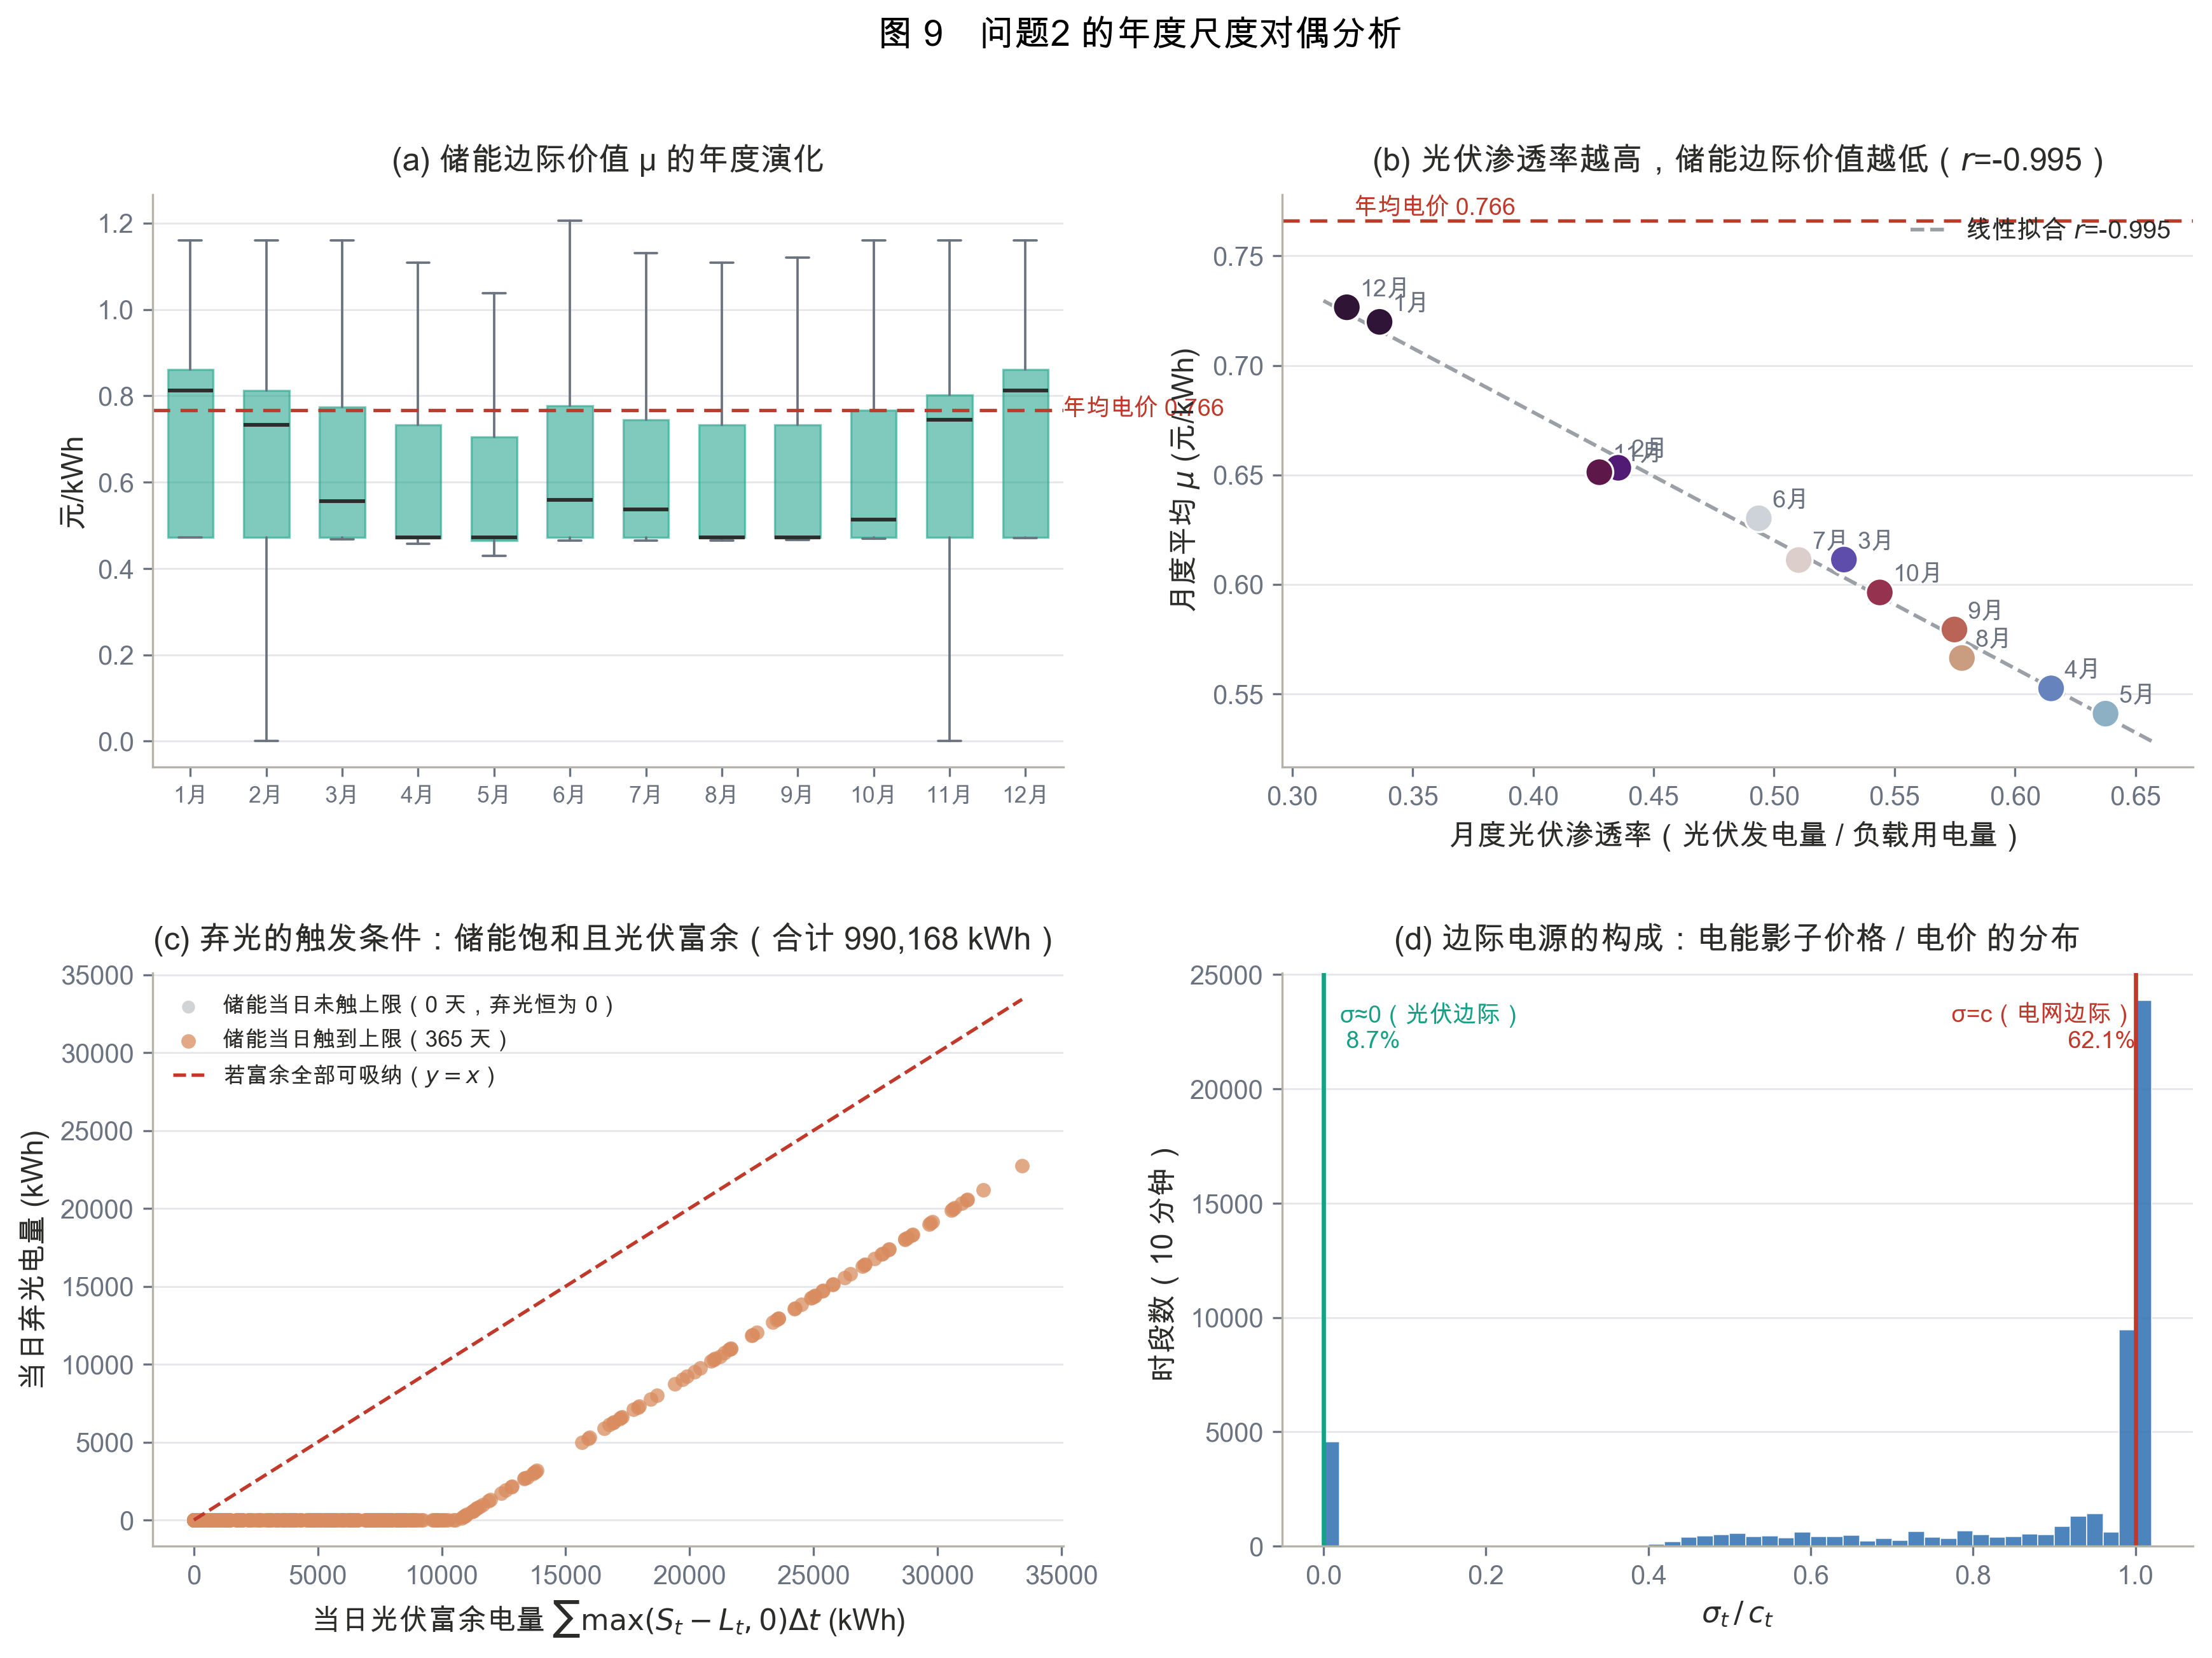
\includegraphics[width=0.98\textwidth]{fig_p2_dual.png}
\caption{问题2 年度对偶演化：(a) 储能边际价值 $\mu_t$ 的月度分布；(b) 渗透率与储能价值负相关；(c) 弃光触发条件；(d) 边际电源排序}\label{fig:p2dual}
\end{figure}

% ================= P2
\begin{table}[H]\centering\small
\caption{问题2：微网在指定日期指定时段的购电量及全天购电量与购电费}\label{tab:p2t1}
\resizebox{\textwidth}{!}{\begin{tabular}{lrrrrrrrr}
\toprule
日期 & 10:00-10:10 & 12:00-12:10 & 14:00-14:10 & 16:00-16:10 & 18:00-18:10 & 20:00-20:10 & 全天购电量 & 全天购电费\\
\midrule
3 月 20 日 & 0.00 & 558.31 & 0.00 & 507.32 & 682.35 & 0.00 & 61,491.9 & 37,889.6\\
6 月 21 日 & 0.00 & 0.00 & 0.00 & 27.01 & 385.90 & 0.00 & 39,100.7 & 20,541.4\\
9 月 23 日 & 0.00 & 380.02 & 0.00 & 493.58 & 752.64 & 0.00 & 66,432.1 & 41,382.7\\
12 月 21 日 & 0.00 & 906.68 & 0.00 & 795.93 & 712.63 & 0.00 & 93,603.5 & 59,593.4\\
\bottomrule\end{tabular}}\end{table}
\begin{table}[H]\centering\small
\caption{问题2：储能设备在指定日期指定时间段的充放电量及储电量}\label{tab:p2t2}
\resizebox{\textwidth}{!}{\begin{tabular}{lrrrrrrrrrrrrr}
\toprule
日期 & 00:00-04:00 & 04:00-08:00 & 08:00-12:00 & 12:00-16:00 & 16:00-20:00 & 20:00-24:00 & \\
 & \multicolumn{1}{c}{充} & \multicolumn{1}{c}{充} & \multicolumn{1}{c}{充} & \multicolumn{1}{c}{充} & \multicolumn{1}{c}{充} & \multicolumn{1}{c}{充} & \multicolumn{1}{c}{0:00 储电量}\\
 & \multicolumn{1}{c}{放} & \multicolumn{1}{c}{放} & \multicolumn{1}{c}{放} & \multicolumn{1}{c}{放} & \multicolumn{1}{c}{放} & \multicolumn{1}{c}{放} & \multicolumn{1}{c}{24:00 储电量}\\
\midrule
3 月 20 日 & 1,500.0 & 833.3 & 6,291.5 & 4,689.7 & 0.0 & 3,503.2 & 8,700\\
 & 0.0 & 5,862.6 & 2,777.4 & 254.7 & 5,709.8 & 2,930.2 & 4,353\\
\midrule
6 月 21 日 & 0.0 & 833.3 & 2,200.8 & 8,465.8 & 0.0 & 8,333.3 & 2,361\\
 & 0.0 & 1,720.0 & 0.0 & 0.0 & 6,154.1 & 2,485.9 & 8,700\\
\midrule
9 月 23 日 & 1,666.7 & 833.3 & 5,245.4 & 5,923.8 & 0.0 & 8,333.3 & 8,550\\
 & 0.0 & 6,746.8 & 1,896.6 & 403.6 & 5,602.9 & 3,037.1 & 8,700\\
\midrule
12 月 21 日 & 1,500.0 & 1,666.7 & 5,833.3 & 7,574.2 & 0.0 & 8,166.7 & 8,700\\
 & 0.0 & 1,508.3 & 7,806.7 & 2,220.1 & 5,797.5 & 2,842.5 & 8,550\\
\bottomrule\end{tabular}}\end{table}

\section{问题3：罚金感知滚动时域优化（MPC-II）}\label{sec:p3}

\subsection{决策结构：一日四检查点}
每日 0:00 以 24 h 预报制定全天计划 $g^0$；6:00/12:00/18:00 各获得更新预报后\textbf{重优化其后时段}（图~\ref{fig:s3}）。计划量 $g^0$ 全额计费（承诺量），重优化只确定调整量 $a$。

\begin{figure}[H]\centering
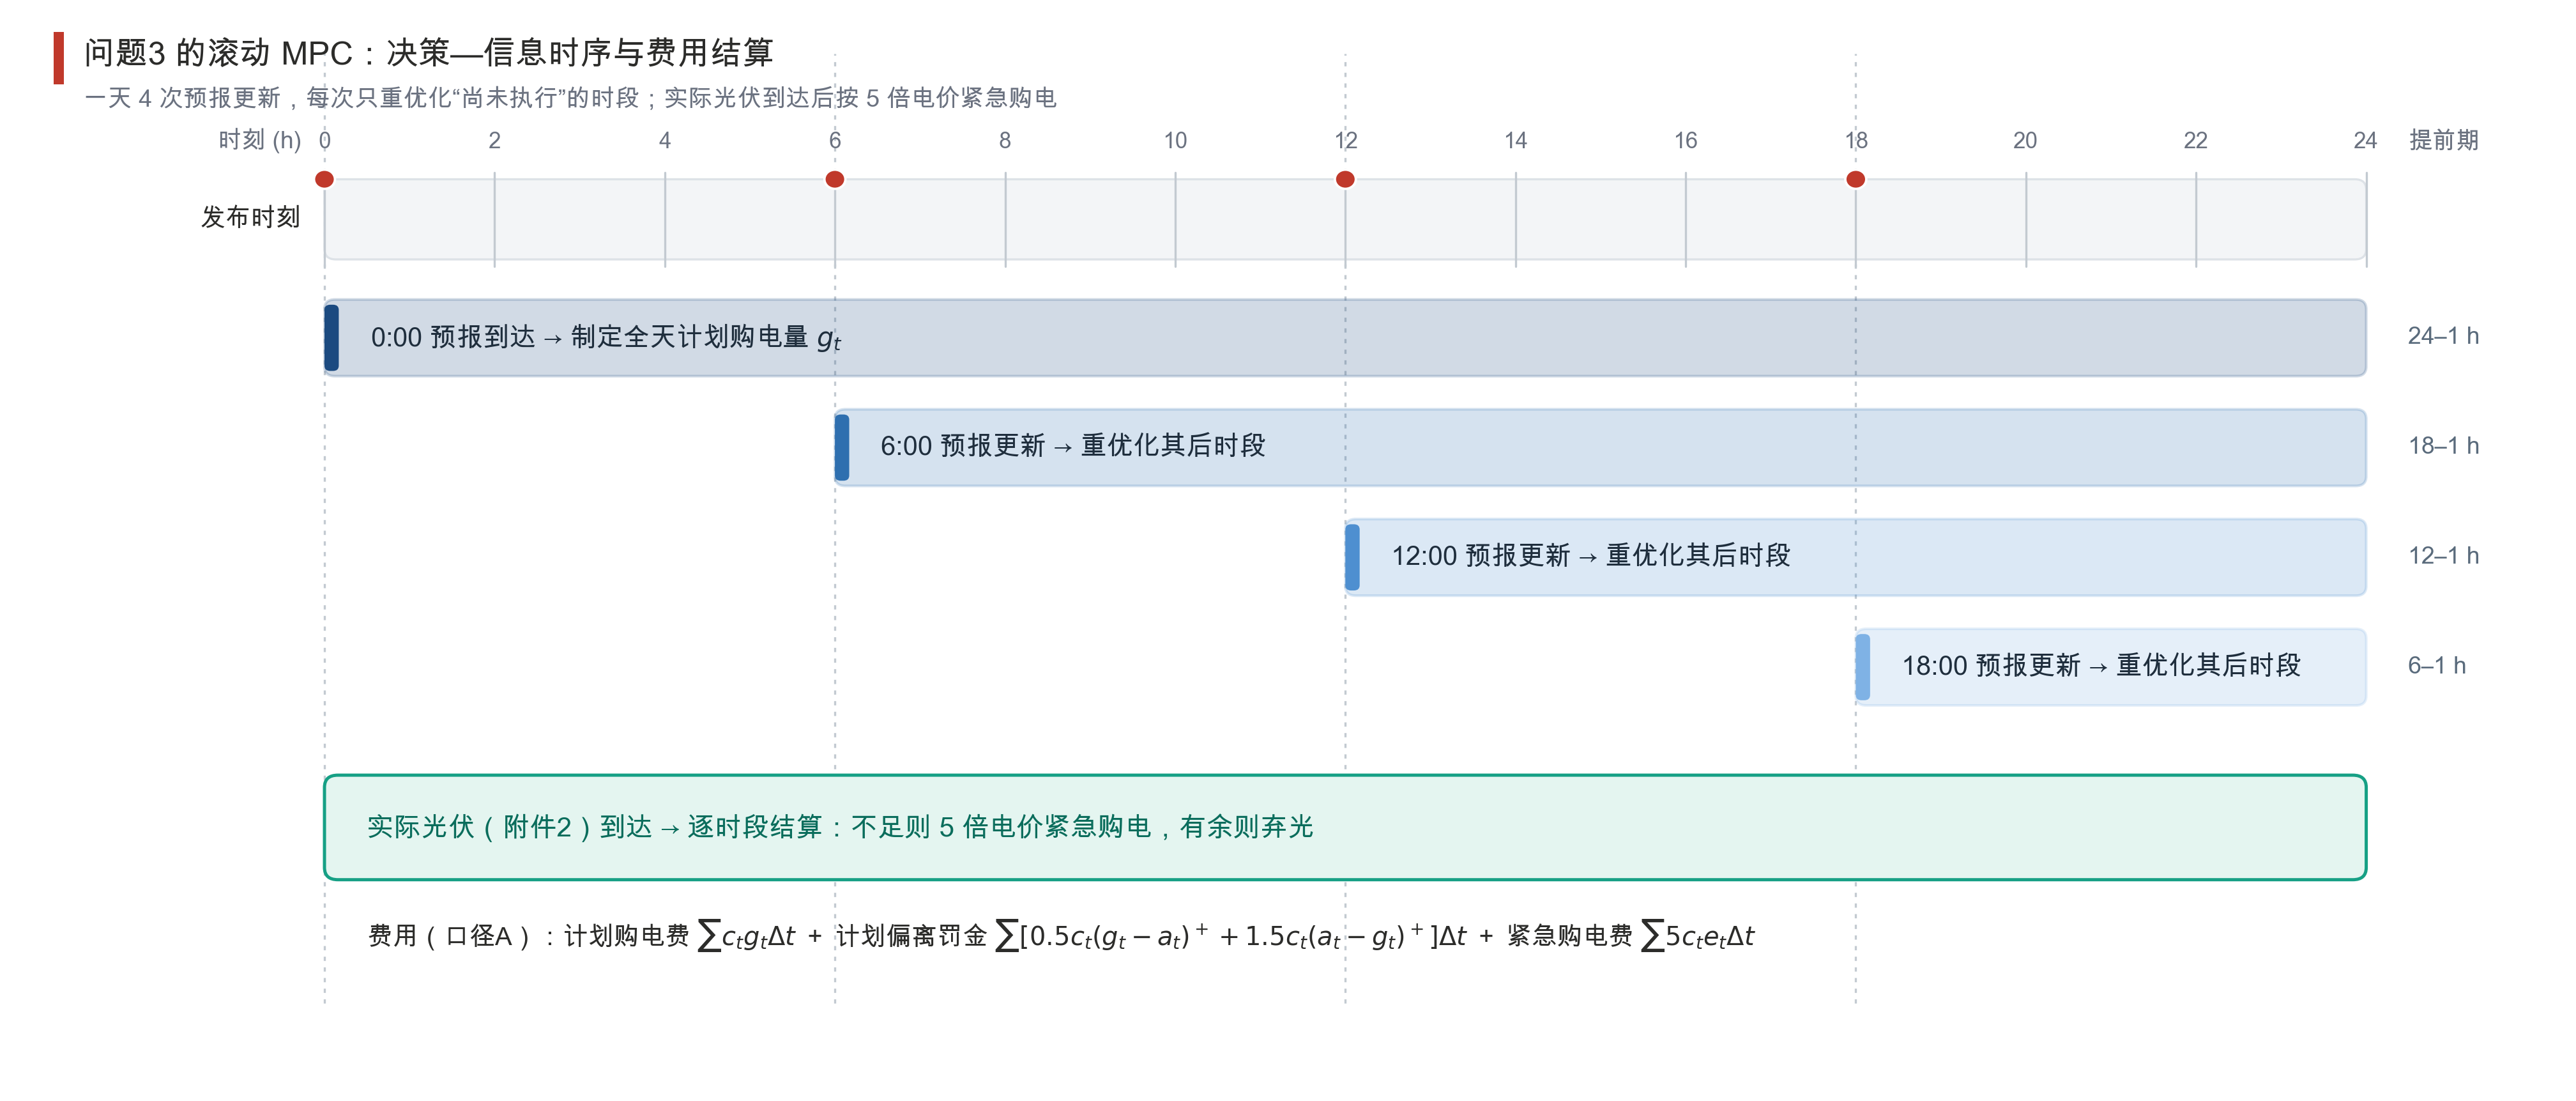
\includegraphics[width=0.98\textwidth]{fig_s3_timeline.png}
\caption{问题3 滚动决策时序：四次预报的覆盖区间与提前期}\label{fig:s3}
\end{figure}

\subsection{★关键建模：子问题的目标函数是罚金，不是购电成本}\label{sec:penalty}
\textbf{先从最朴素的滚动优化出发}：每个检查点把重优化当作一次普通购电决策，目标为 $\min\sum c_t a_t\Delta t$——为建模简便，暂不区分计划与调整的费用差异。然而题面规定\textbf{除紧急购电费用外，购电费用\textbf{均按计划购电量}计算}，即 $g^0$ 是已按 $c_t$ 全额付费的\textbf{承诺量}；于是重优化中购电费早已锁定，\textbf{调整的边际成本只能是罚金而非购电成本}：
\begin{align}
\min_{a_t,u_t,v_t}\ &\sum_{t\ge s}\Big[0.5\,c_t\,d^{-}_t+1.5\,c_t\,d^{+}_t\Big]\Delta t\label{eq:penobj}\\
\text{s.t.}\quad & d^{-}_t-d^{+}_t+a_t=g^0_t,\ d^{-}_t,d^{+}_t\ge0\ (\text{线性化取大}),\ \text{及功率平衡、储能动态约束}.\nonumber
\end{align}
上述朴素基线恰好等价于\textbf{假定调整免费}，LP 于是肆意重优化：实测调整偏离总量高达 113.95 万 kWh、罚金 66.3 万元（对照结果见 \S\ref{sec:p3} 与图~\ref{fig:ladder}）。修正后的子问题引入每时段 2 个辅助变量，\eqref{eq:penobj} 仍为 LP；0:00 子问题的目标本就是计划购电费用，保持不变。至此形成方法链的中间层：\textbf{朴素 MPC（简化基线）$\to$ 罚金感知修正（MPC-II）}，其与策略最优上限的距离由 SDP 给出（\S\ref{sec:sdp}）。

\subsection{执行与结算仿真}
每日执行采用\textbf{计划 $\to$ 调整 $\to$ 实际}三段仿真：以调整后的购电量为承诺执行，实际光伏 $S$ 结算：
\[
\text{短缺}\ \mathrm{emg}_t=\max(L_t+u_t-v_t-S_t-a_t,0)\times 5c_t,\qquad
\text{弃光}\ w_t=\max(S_t+a_t+v_t-L_t-u_t,0).
\]
交付期费用（口径A，334 天）：
\[
\underbrace{12\,385\,349.09}_{\text{计划购电}}+
\underbrace{432\,689.71}_{\text{调整罚金}}+
\underbrace{1\,074\,066.10}_{\text{紧急购电}}
=\boxed{13\,892\,104.90\ \text{元}}.
\]
对照朴素 MPC（子问题目标为购电成本）：总费用 14\,248\,837.72 元，\textbf{MPC-II 节省 356\,733 元（2.50\%）}，调整偏离总量 113.95 万$\to$44.38 万 kWh（$-61\%$）。全年滚动共求解 $334\times4=1336$ 个 LP。

\subsection{预报的信息价值}
仅用 0:00 预报费用为 14\,756\,862.50 元；追加 6:00/12:00/18:00 三次预报节省 \textbf{864\,758 元（5.86\%）}，紧急购电量由 59.2 万降至 26.2 万 kWh。但距完美信息（12\,245\,046.92 元）仍差 \textbf{13.45\%}——信息质量的改进空间远大于决策频次（\S\ref{sec:sdp} 量化）。题面要求的指定日期结果见表~\ref{tab:p3t1}--\ref{tab:p3t2}，全年形态见图~\ref{fig:p3}。

\begin{figure}[H]\centering
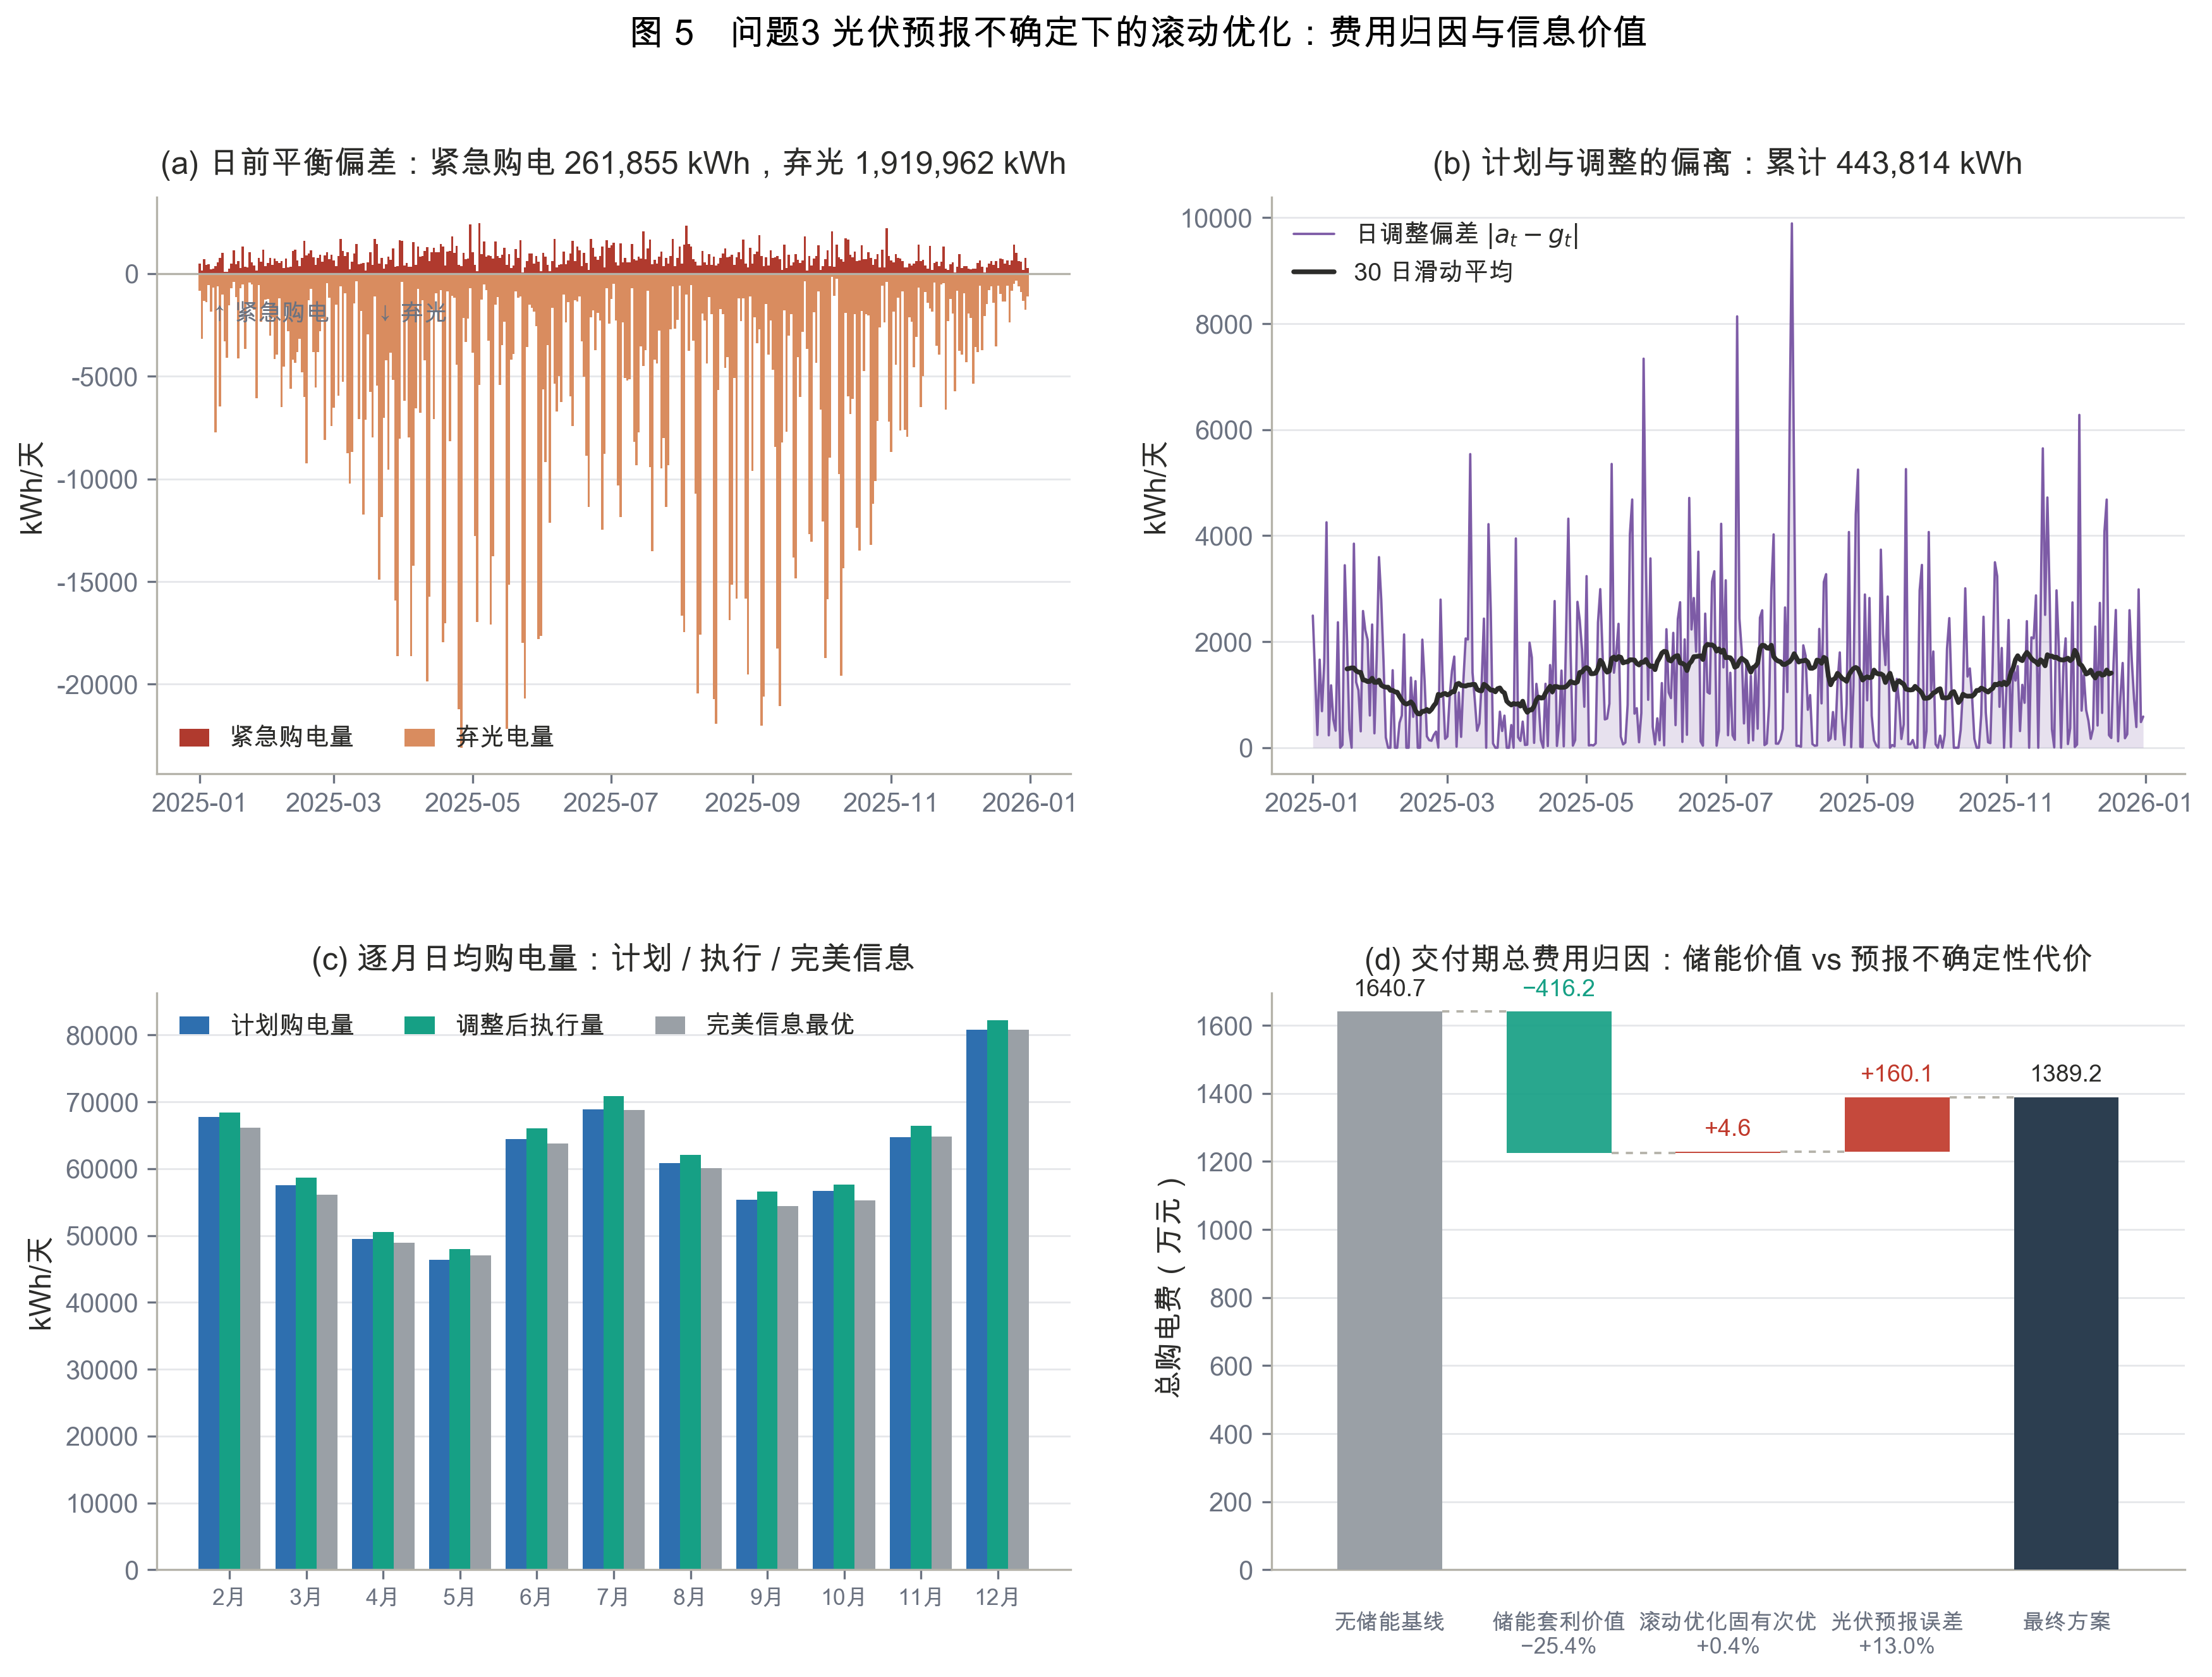
\includegraphics[width=0.98\textwidth]{fig_p3_rolling.png}
\caption{问题3 滚动优化结果：(a) 日前平衡偏差；(b) 紧急购电分布；(c) 月度费用构成；(d) 成本归因瀑布图}\label{fig:p3}
\end{figure}

% ================= P3
\begin{table}[H]\centering\small
\caption{问题3：微网在指定日期指定时段的购电量及全天购电量与购电费}\label{tab:p3t1}
\resizebox{\textwidth}{!}{\begin{tabular}{lrrrrrrrrr}
\toprule
日期 & 10:00-10:10 & 12:00-12:10 & 14:00-14:10 & 16:00-16:10 & 18:00-18:10 & 20:00-20:10 & 全天购电量 & 全天购电费 & 紧急购电量\\
\midrule
3 月 20 日 & 0.00 & 553.56 & 0.00 & 641.13 & 682.35 & 0.00 & 70,316.7 & 50,333.3 & 1,446.7\\
6 月 21 日 & 0.00 & 0.00 & 0.00 & 112.92 & 396.16 & 0.00 & 33,508.2 & 19,229.2 & 172.8\\
9 月 23 日 & 0.00 & 358.67 & 0.00 & 550.19 & 752.64 & 0.00 & 68,434.7 & 45,558.9 & 628.3\\
12 月 21 日 & 0.00 & 954.54 & 0.00 & 806.74 & 712.63 & 0.00 & 94,583.0 & 62,719.0 & 494.2\\
\bottomrule\end{tabular}}\end{table}
\begin{table}[H]\centering\small
\caption{问题3：储能设备在指定日期指定时间段的充放电量及储电量}\label{tab:p3t2}
\resizebox{\textwidth}{!}{\begin{tabular}{lrrrrrrrrrrrrr}
\toprule
日期 & 00:00-04:00 & 04:00-08:00 & 08:00-12:00 & 12:00-16:00 & 16:00-20:00 & 20:00-24:00 & \\
 & \multicolumn{1}{c}{充} & \multicolumn{1}{c}{充} & \multicolumn{1}{c}{充} & \multicolumn{1}{c}{充} & \multicolumn{1}{c}{充} & \multicolumn{1}{c}{充} & \multicolumn{1}{c}{0:00 储电量}\\
 & \multicolumn{1}{c}{放} & \multicolumn{1}{c}{放} & \multicolumn{1}{c}{放} & \multicolumn{1}{c}{放} & \multicolumn{1}{c}{放} & \multicolumn{1}{c}{放} & \multicolumn{1}{c}{24:00 储电量}\\
\midrule
3 月 20 日 & 4,500.0 & 833.3 & 684.4 & 9,778.9 & 472.7 & 5,333.3 & 6,000\\
 & 0.0 & 6,380.7 & 2,259.3 & 218.2 & 5,709.8 & 2,930.2 & 6,000\\
\midrule
6 月 21 日 & 0.0 & 0.0 & 1,585.6 & 8,651.9 & 149.5 & 5,333.3 & 6,000\\
 & 0.0 & 4,093.4 & 0.0 & 0.0 & 6,154.1 & 2,485.9 & 6,000\\
\midrule
9 月 23 日 & 4,500.0 & 833.3 & 4,853.7 & 5,815.0 & 302.9 & 5,333.3 & 6,000\\
 & 0.0 & 6,743.9 & 1,812.0 & 331.2 & 5,602.9 & 3,037.1 & 6,000\\
\midrule
12 月 21 日 & 4,500.0 & 1,244.6 & 6,044.3 & 7,500.0 & 0.0 & 5,333.3 & 6,000\\
 & 0.0 & 1,514.3 & 7,361.9 & 2,427.8 & 5,797.5 & 2,842.5 & 6,000\\
\bottomrule\end{tabular}}\end{table}

\section{问题4：波动电价下的双轨决策}\label{sec:p4}

\subsection{双轨结构}
将\textbf{电价信息}从光伏信息中剥离，形成 $2\times2$ 矩阵（图~\ref{fig:s4}）：轨一为完美信息上界（4-2 整年 LP、4-3 滚动调整）；轨二假设电价不可预知，\textbf{决策只能用历史分时均价 $\bar c_t$（附件1）}，结算按附件4 实际电价。两轨之差即电价不确定性的精确价格。

\begin{figure}[H]\centering
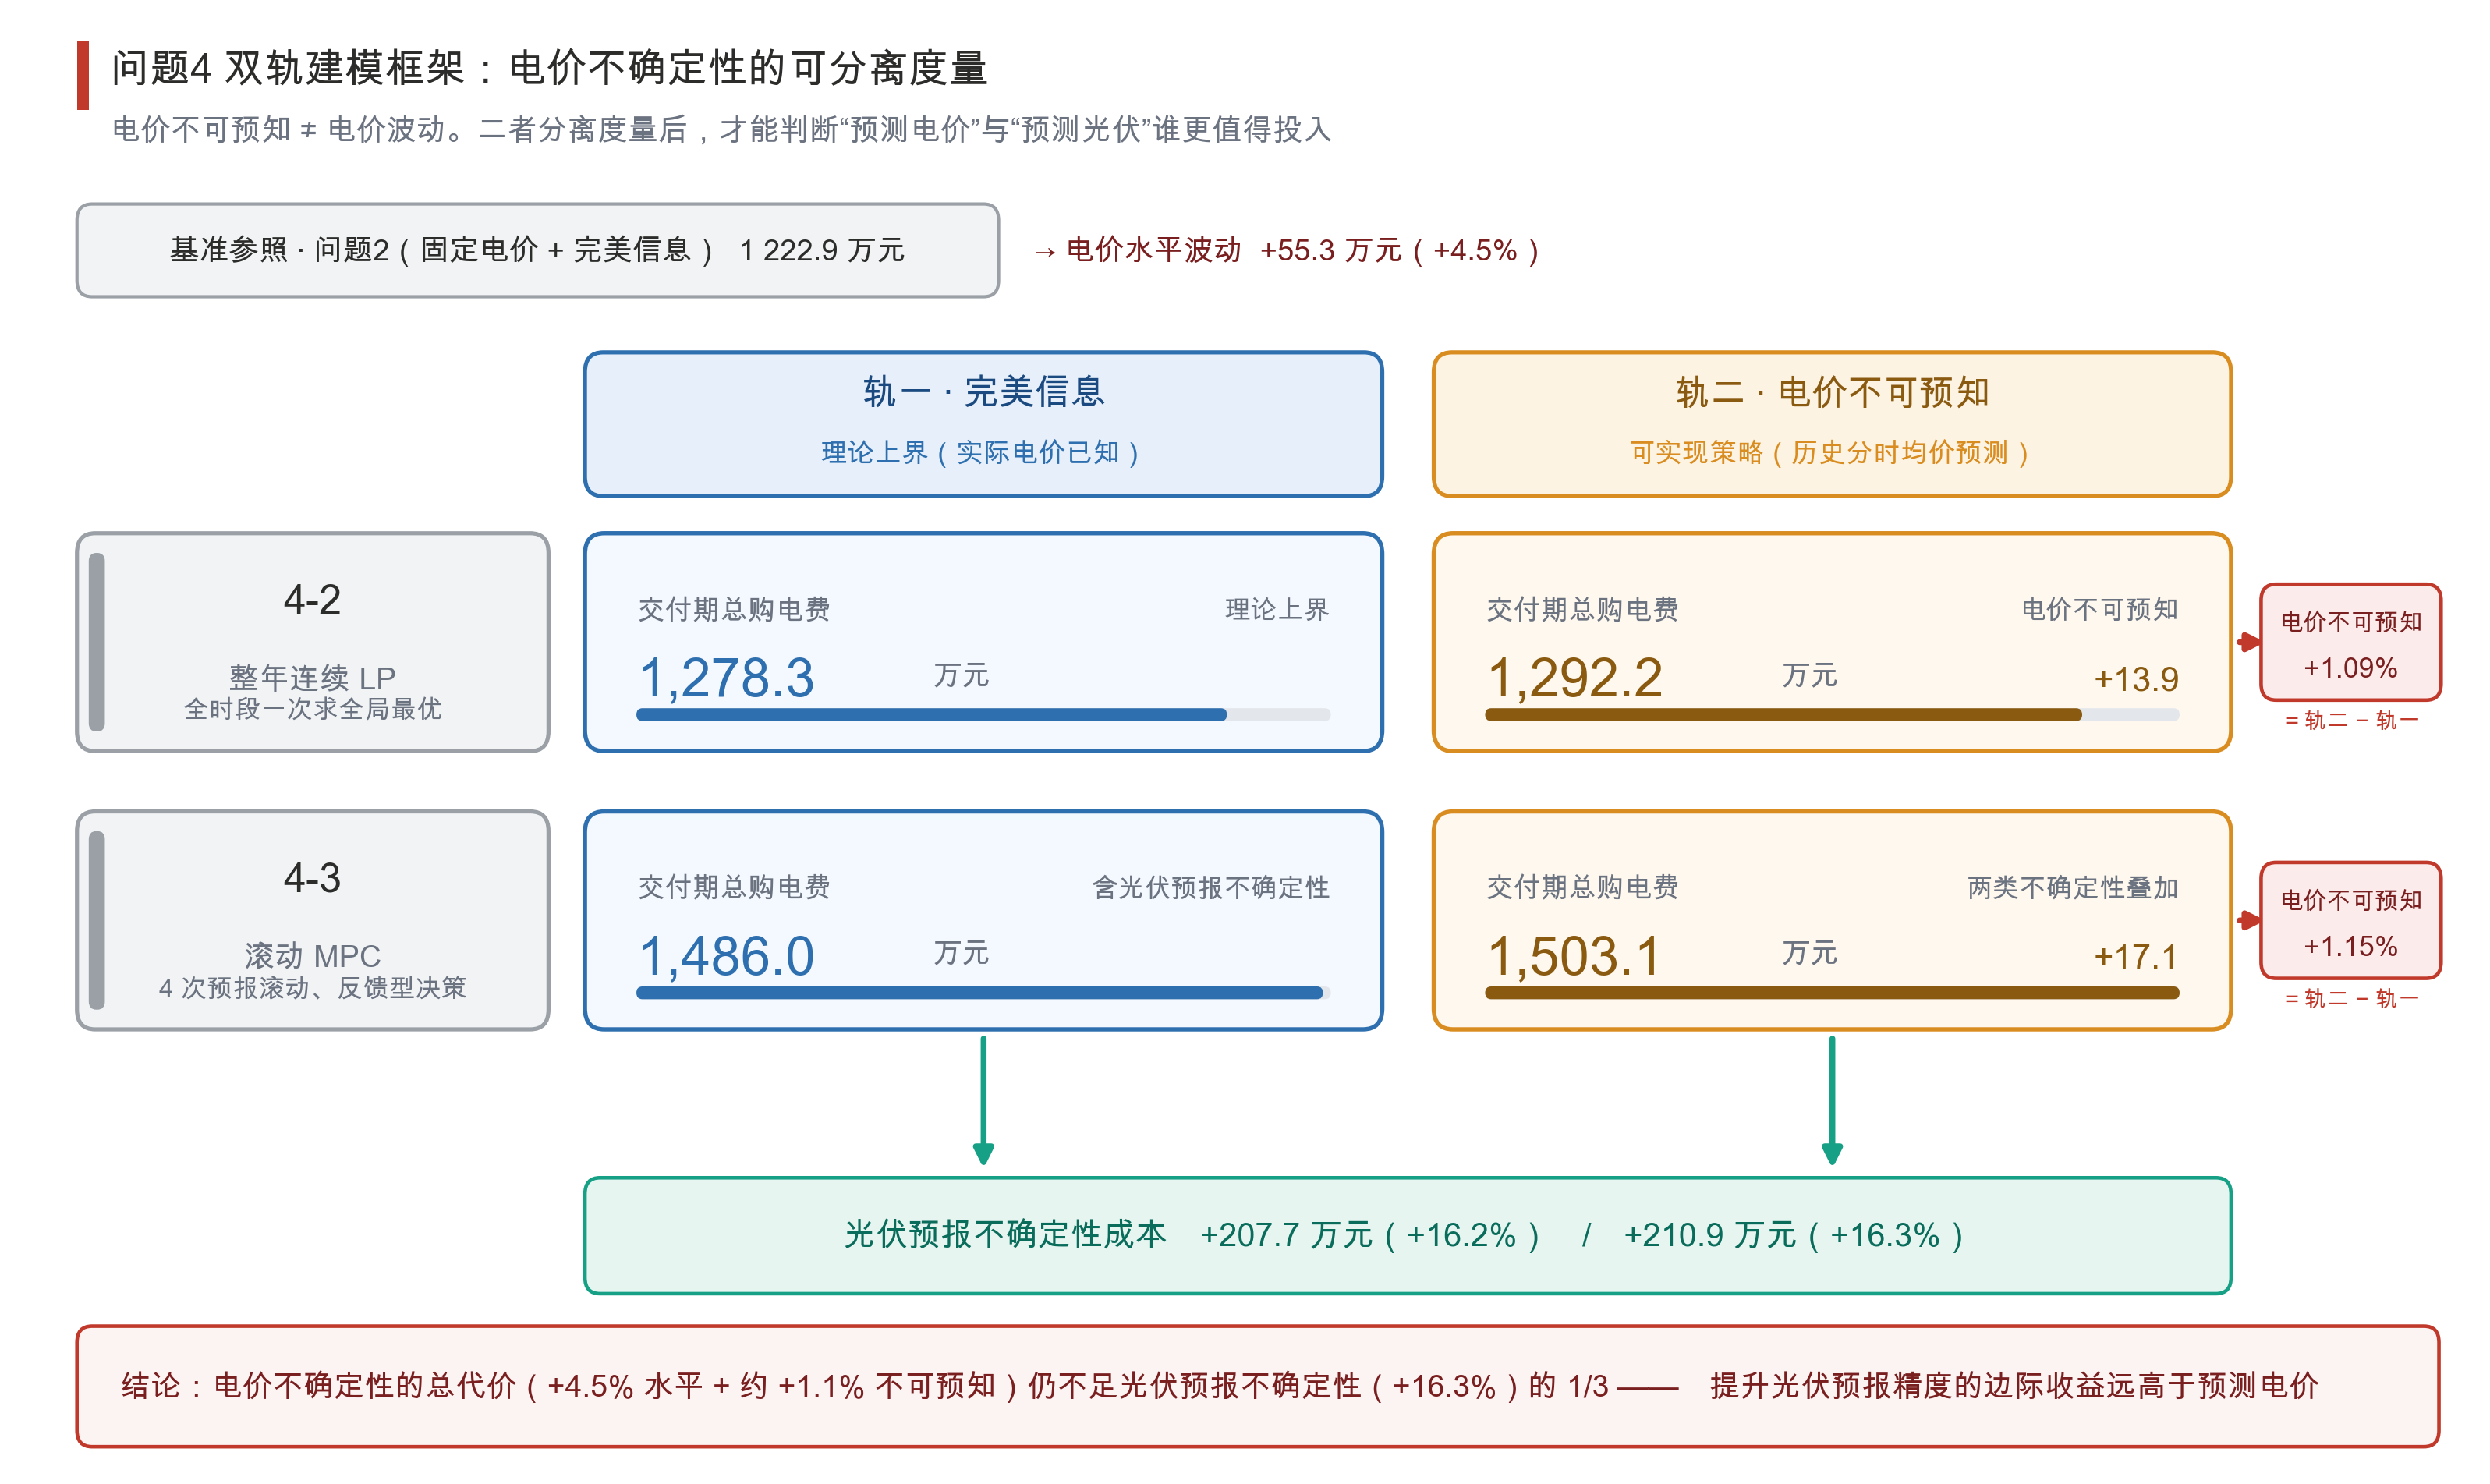
\includegraphics[width=0.98\textwidth]{fig_s4_framework.png}
\caption{问题4 双轨框架：行 = 决策方法，列 = 电价信息假设}\label{fig:s4}
\end{figure}

\subsection{结果}
\begin{table}[H]\centering\small
\caption{问题4 双轨结果（交付期 334 天）}\label{tab:p4}
\begin{tabular}{lrr}
\toprule
轨 & 4-2 整年 LP & 4-3 滚动调整（MPC-II）\\
\midrule
轨一（电价完美信息） & 12\,782\,591.81 & 14\,526\,493.69\\
轨二（电价不可预知） & 12\,922\,053.07 & 14\,649\,148.30\\
\midrule
\textbf{电价不确定性成本} & 139\,461.26（1.09\%） & 122\,654.62（\textbf{0.84\%}）\\
\bottomrule
\end{tabular}
\end{table}

4-3 轨一的构成：计划购电 12\,966\,547.11 + 调整罚金 464\,755.44 + 紧急购电 1\,095\,191.13 元。与问题3 同口径对比：波动电价的\textbf{水平效应}使 4-2 较问题2 上升 553\,131 元（$+4.52\%$）、4-3 较问题3 上升 634\,389 元（$+4.57\%$）。叠加后，电价总效应（约 5.4\%）仍\textbf{不足光伏预报不确定性（13.45\%）的一半}：储能的削峰填谷对电价波动具有天然鲁棒性，而预报误差直接击穿日前平衡（图~\ref{fig:p4}）。表~\ref{tab:p42t1}--\ref{tab:p43t2} 与表~\ref{tab:p4t3} 给出题面要求的指定日期明细。

\begin{figure}[H]\centering
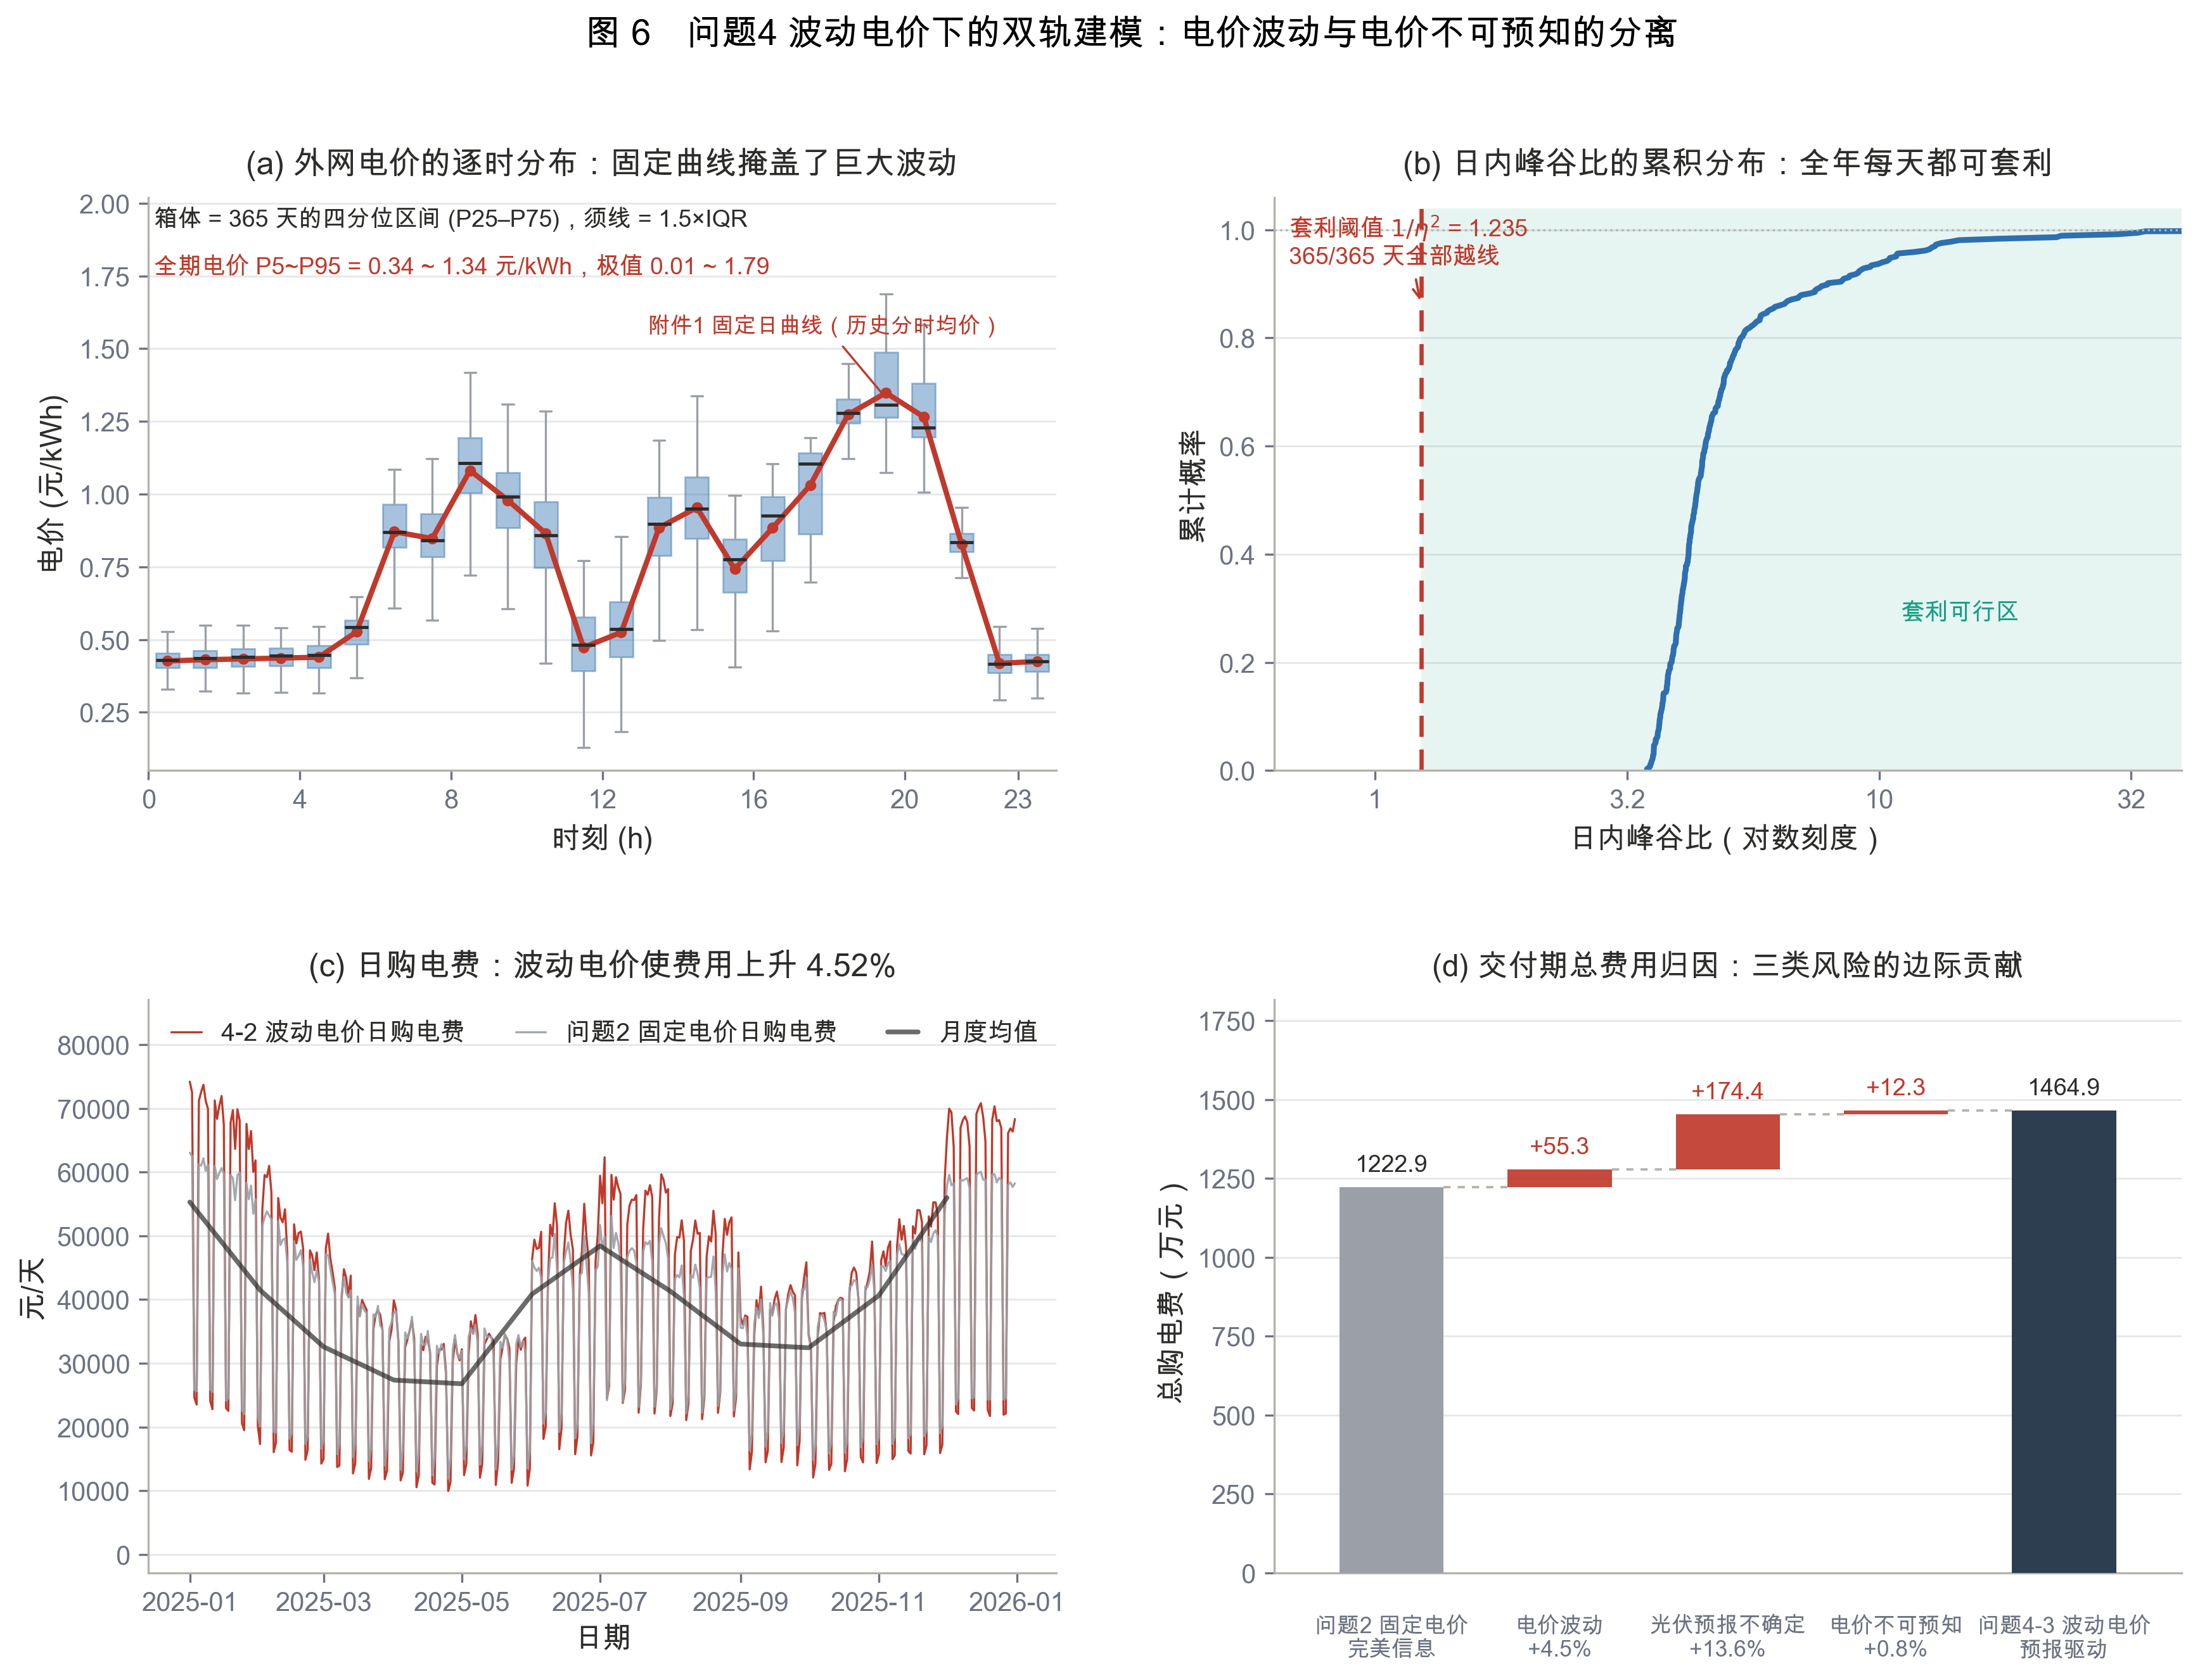
\includegraphics[width=0.98\textwidth]{fig_p4_price.png}
\caption{问题4：(a) 电价逐时分布箱线图；(b) 峰谷比累积分布；(c) 轨一 vs 轨二日费用；(d) 三类风险的成本归因瀑布图}\label{fig:p4}
\end{figure}

% ================= P42
\begin{table}[H]\centering\small
\caption{问题4-2（完美信息）：微网在指定日期指定时段的购电量及全天购电量与购电费}\label{tab:p42t1}
\resizebox{\textwidth}{!}{\begin{tabular}{lrrrrrrrr}
\toprule
日期 & 10:00-10:10 & 12:00-12:10 & 14:00-14:10 & 16:00-16:10 & 18:00-18:10 & 20:00-20:10 & 全天购电量 & 全天购电费\\
\midrule
3 月 20 日 & 0.00 & 558.31 & 0.00 & 507.32 & 682.35 & 726.37 & 60,808.5 & 38,385.8\\
6 月 21 日 & 0.00 & 0.00 & 0.00 & 27.01 & 385.90 & 0.00 & 40,707.5 & 18,491.8\\
9 月 23 日 & 0.00 & 380.02 & 0.00 & 493.58 & 752.64 & 265.83 & 65,265.4 & 42,272.8\\
12 月 21 日 & 0.00 & 906.68 & 0.00 & 795.93 & 712.63 & 0.00 & 90,270.2 & 68,224.3\\
\bottomrule\end{tabular}}\end{table}
\begin{table}[H]\centering\small
\caption{问题4-2（完美信息）：储能设备在指定日期指定时间段的充放电量及储电量}\label{tab:p42t2}
\resizebox{\textwidth}{!}{\begin{tabular}{lrrrrrrrrrrrrr}
\toprule
日期 & 00:00-04:00 & 04:00-08:00 & 08:00-12:00 & 12:00-16:00 & 16:00-20:00 & 20:00-24:00 & \\
 & \multicolumn{1}{c}{充} & \multicolumn{1}{c}{充} & \multicolumn{1}{c}{充} & \multicolumn{1}{c}{充} & \multicolumn{1}{c}{充} & \multicolumn{1}{c}{充} & \multicolumn{1}{c}{0:00 储电量}\\
 & \multicolumn{1}{c}{放} & \multicolumn{1}{c}{放} & \multicolumn{1}{c}{放} & \multicolumn{1}{c}{放} & \multicolumn{1}{c}{放} & \multicolumn{1}{c}{放} & \multicolumn{1}{c}{24:00 储电量}\\
\midrule
3 月 20 日 & 1,666.7 & 2,500.0 & 6,291.5 & 4,662.1 & 0.0 & 1,666.7 & 7,050\\
 & 0.0 & 5,840.3 & 2,777.4 & 254.7 & 6,412.3 & 2,902.7 & 1,950\\
\midrule
6 月 21 日 & 1,666.7 & 2,123.4 & 701.6 & 9,965.1 & 0.0 & 8,333.3 & 1,200\\
 & 1,350.0 & 1,720.0 & 0.0 & 0.0 & 6,154.1 & 2,485.9 & 8,700\\
\midrule
9 月 23 日 & 4,166.7 & 3,166.7 & 5,070.5 & 6,098.6 & 0.0 & 2,333.3 & 4,200\\
 & 0.0 & 6,746.8 & 1,896.6 & 403.6 & 7,021.8 & 1,618.2 & 3,300\\
\midrule
12 月 21 日 & 666.7 & 833.3 & 5,833.3 & 7,500.0 & 74.2 & 6,500.0 & 10,200\\
 & 0.0 & 1,508.3 & 7,806.7 & 2,220.1 & 5,171.9 & 3,468.1 & 7,050\\
\bottomrule\end{tabular}}\end{table}
% ================= P43
\begin{table}[H]\centering\small
\caption{问题4-3（滚动调整）：微网在指定日期指定时段的购电量及全天购电量与购电费}\label{tab:p43t1}
\resizebox{\textwidth}{!}{\begin{tabular}{lrrrrrrrrr}
\toprule
日期 & 10:00-10:10 & 12:00-12:10 & 14:00-14:10 & 16:00-16:10 & 18:00-18:10 & 20:00-20:10 & 全天购电量 & 全天购电费 & 紧急购电量\\
\midrule
3 月 20 日 & 0.00 & 553.56 & 0.00 & 641.13 & 682.35 & 726.37 & 70,303.2 & 51,535.3 & 1,466.8\\
6 月 21 日 & 0.00 & 0.00 & 0.00 & 112.92 & 396.16 & 0.00 & 34,098.7 & 16,525.3 & 172.8\\
9 月 23 日 & 0.00 & 358.67 & 0.00 & 550.19 & 752.64 & 266.57 & 68,434.7 & 47,169.1 & 657.9\\
12 月 21 日 & 0.00 & 954.54 & 0.00 & 806.74 & 712.63 & 0.00 & 94,549.0 & 73,018.2 & 370.6\\
\bottomrule\end{tabular}}\end{table}
\begin{table}[H]\centering\small
\caption{问题4-3（滚动调整）：储能设备在指定日期指定时间段的充放电量及储电量}\label{tab:p43t2}
\resizebox{\textwidth}{!}{\begin{tabular}{lrrrrrrrrrrrrr}
\toprule
日期 & 00:00-04:00 & 04:00-08:00 & 08:00-12:00 & 12:00-16:00 & 16:00-20:00 & 20:00-24:00 & \\
 & \multicolumn{1}{c}{充} & \multicolumn{1}{c}{充} & \multicolumn{1}{c}{充} & \multicolumn{1}{c}{充} & \multicolumn{1}{c}{充} & \multicolumn{1}{c}{充} & \multicolumn{1}{c}{0:00 储电量}\\
 & \multicolumn{1}{c}{放} & \multicolumn{1}{c}{放} & \multicolumn{1}{c}{放} & \multicolumn{1}{c}{放} & \multicolumn{1}{c}{放} & \multicolumn{1}{c}{放} & \multicolumn{1}{c}{24:00 储电量}\\
\midrule
3 月 20 日 & 2,000.0 & 3,333.3 & 657.4 & 9,667.1 & 472.7 & 5,333.3 & 6,000\\
 & 0.0 & 6,380.7 & 2,259.3 & 105.7 & 6,412.3 & 2,227.7 & 6,000\\
\midrule
6 月 21 日 & 833.3 & 2,274.6 & 1,768.0 & 8,469.5 & 149.5 & 5,333.3 & 6,000\\
 & 4,995.0 & 1,615.8 & 0.0 & 0.0 & 6,154.1 & 2,485.9 & 6,000\\
\midrule
9 月 23 日 & 2,833.3 & 2,500.0 & 4,357.3 & 6,311.4 & 302.9 & 5,333.3 & 6,000\\
 & 0.0 & 6,743.9 & 1,812.0 & 331.2 & 7,021.8 & 1,618.2 & 6,000\\
\midrule
12 月 21 日 & 5,333.3 & 833.3 & 5,602.4 & 7,500.0 & 0.0 & 5,333.3 & 6,000\\
 & 0.0 & 1,516.9 & 7,309.2 & 2,461.8 & 5,171.9 & 3,468.1 & 6,000\\
\bottomrule\end{tabular}}\end{table}
% ================= 表3 紧急购电量
\begin{table}[H]\centering\small
\caption{微网在指定日期的紧急购电量（kWh）}\label{tab:p4t3}
\begin{tabular}{lrr}
\toprule
日期 & 问题3（固定电价） & 问题4（波动电价）\\
\midrule
3 月 20 日 & 1,446.66 & 1,466.77\\
6 月 21 日 & 172.79 & 172.79\\
9 月 23 日 & 628.33 & 657.93\\
12 月 21 日 & 494.18 & 370.56\\
\bottomrule\end{tabular}\end{table}

\section{SDP：策略最优性基准与改进分解}\label{sec:sdp}

问题3 的交付方案已经确定，但\textbf{"它距离同信息结构下的策略最优还有多远"无法由滚动优化自身回答}——需要一类能刻画全体策略的模型作为参照。本文以 SDP 承担这一角色：它不用于交付，而是\textbf{策略最优性基准}，用以检验 MPC-II 的修正方向并量化剩余改进空间。

就措辞的严谨性需作说明：由 Bellman 最优性原理，SDP 在其\textbf{离散化问题内}给出精确最优策略，这一定理严格成立（参见文献[3]）；但相对原连续问题，动作网格（250 kW）收缩了可行域、状态网格与经验分位点数引入近似，SDP 的费用只会被高估，且本文未给出离散化误差的严格证明。因此 SDP 在全文中定位为\textbf{最优性基准}而非最优性证明，下文的 0.16\% 均指同信息结构、同结算口径下的实测差距。

\subsection{可行性：一维状态与闭式结构}
本题状态\textbf{恰为储电量一维}，\textbf{维数灾难}不成立：状态网格 97 点 $\times$ 动作 41 点（250 kW 步长）$\times$ 144 阶段 $\times$ 365 天，纯 numpy 向量化\textbf{全程 30 秒}。进一步，题面的 take-or-pay 结构使成本关于决策为凸分段线性，其导数断点恰为 $\{0,g^0_t\}\cup\{A_t+\varepsilon_m\}$（$A_t=L_t+u_t-v_t-\hat S_t$ 为净需求中心，与状态解耦），故最优计划可对每个 $(t,\text{动作})$ \textbf{闭式}求得——这把 SDP 压缩为查表。

\subsection{Bellman 方程与两个反直觉结论}
\[
V_t(E)=\min_{g_t}\ \E_{\varepsilon}\Big[c_tg_t+\mathrm{pen}_t(g_t,g^0_t)+5c_t\,\big(\text{net}_t-g_t\big)^+\ \Big|\ E\Big]+V_{t+1}\!\big(E+\eta\Delta t\,u-\tfrac{\Delta t}{\eta}v\big),
\]
其中预报误差 $\varepsilon$ 取自按提前期与预报水平分箱的\textbf{经验分位库}（整日分块自举保持日内相关性）。SDP 解得基准费用 \textbf{13\,869\,883.17 元}，并拆分出两个用 MPC 拿不到的结论：
\begin{enumerate}[label=(\arabic*)]
  \item \textbf{罚金感知是大头（$-2.87\%$）}：正是 \S\ref{sec:penalty} 的缺陷由 SDP 照出。修正后的 MPC-II（$-2.50\%$）已吸收其中绝大部分，距策略最优仅 \textbf{0.16\%（2.2 万元）}；
  \item \textbf{分布感知反而 $-0.22\%$（不省钱），却把紧急购电砍掉 64\%}：安全边际须在高价时段买入，价值只在真缺电时兑现，两者在本数据上几乎抵消——\textbf{可修订性（罚金机制）已替代了安全边际的作用}。理论上由报童逻辑推出的闭式最优计划分位 $g^*=q_{0.727}(\text{net})$ 亦被实测扫描否决（$p=0.50\to0.90$ 费用单调上升 1389.2$\to$1467.2 万元）。
\end{enumerate}

\subsection{决策方法 vs 预报精度}
SDP 上界使两类改进空间\textbf{首次可分离量化}（图~\ref{fig:ladder}）：
\[
\underbrace{2.66\%}_{\text{决策方法：朴素 MPC $\to$ 策略最优}}
\qquad\text{vs}\qquad
\underbrace{13.27\%}_{\text{预报精度：策略最优 $\to$ 完美信息}}.
\]
这是对题面\textbf{是否需要引入其他时刻预报}最有力的回答：\textbf{投资预报，而非投资算法}。交付结果仍用 MPC-II：SDP 的动作离散到 250 kW 网格且优势仅 0.16\%，而 MPC-II 连续、可复现、贴合题目\textbf{计划/调整}措辞。

\begin{figure}[H]\centering
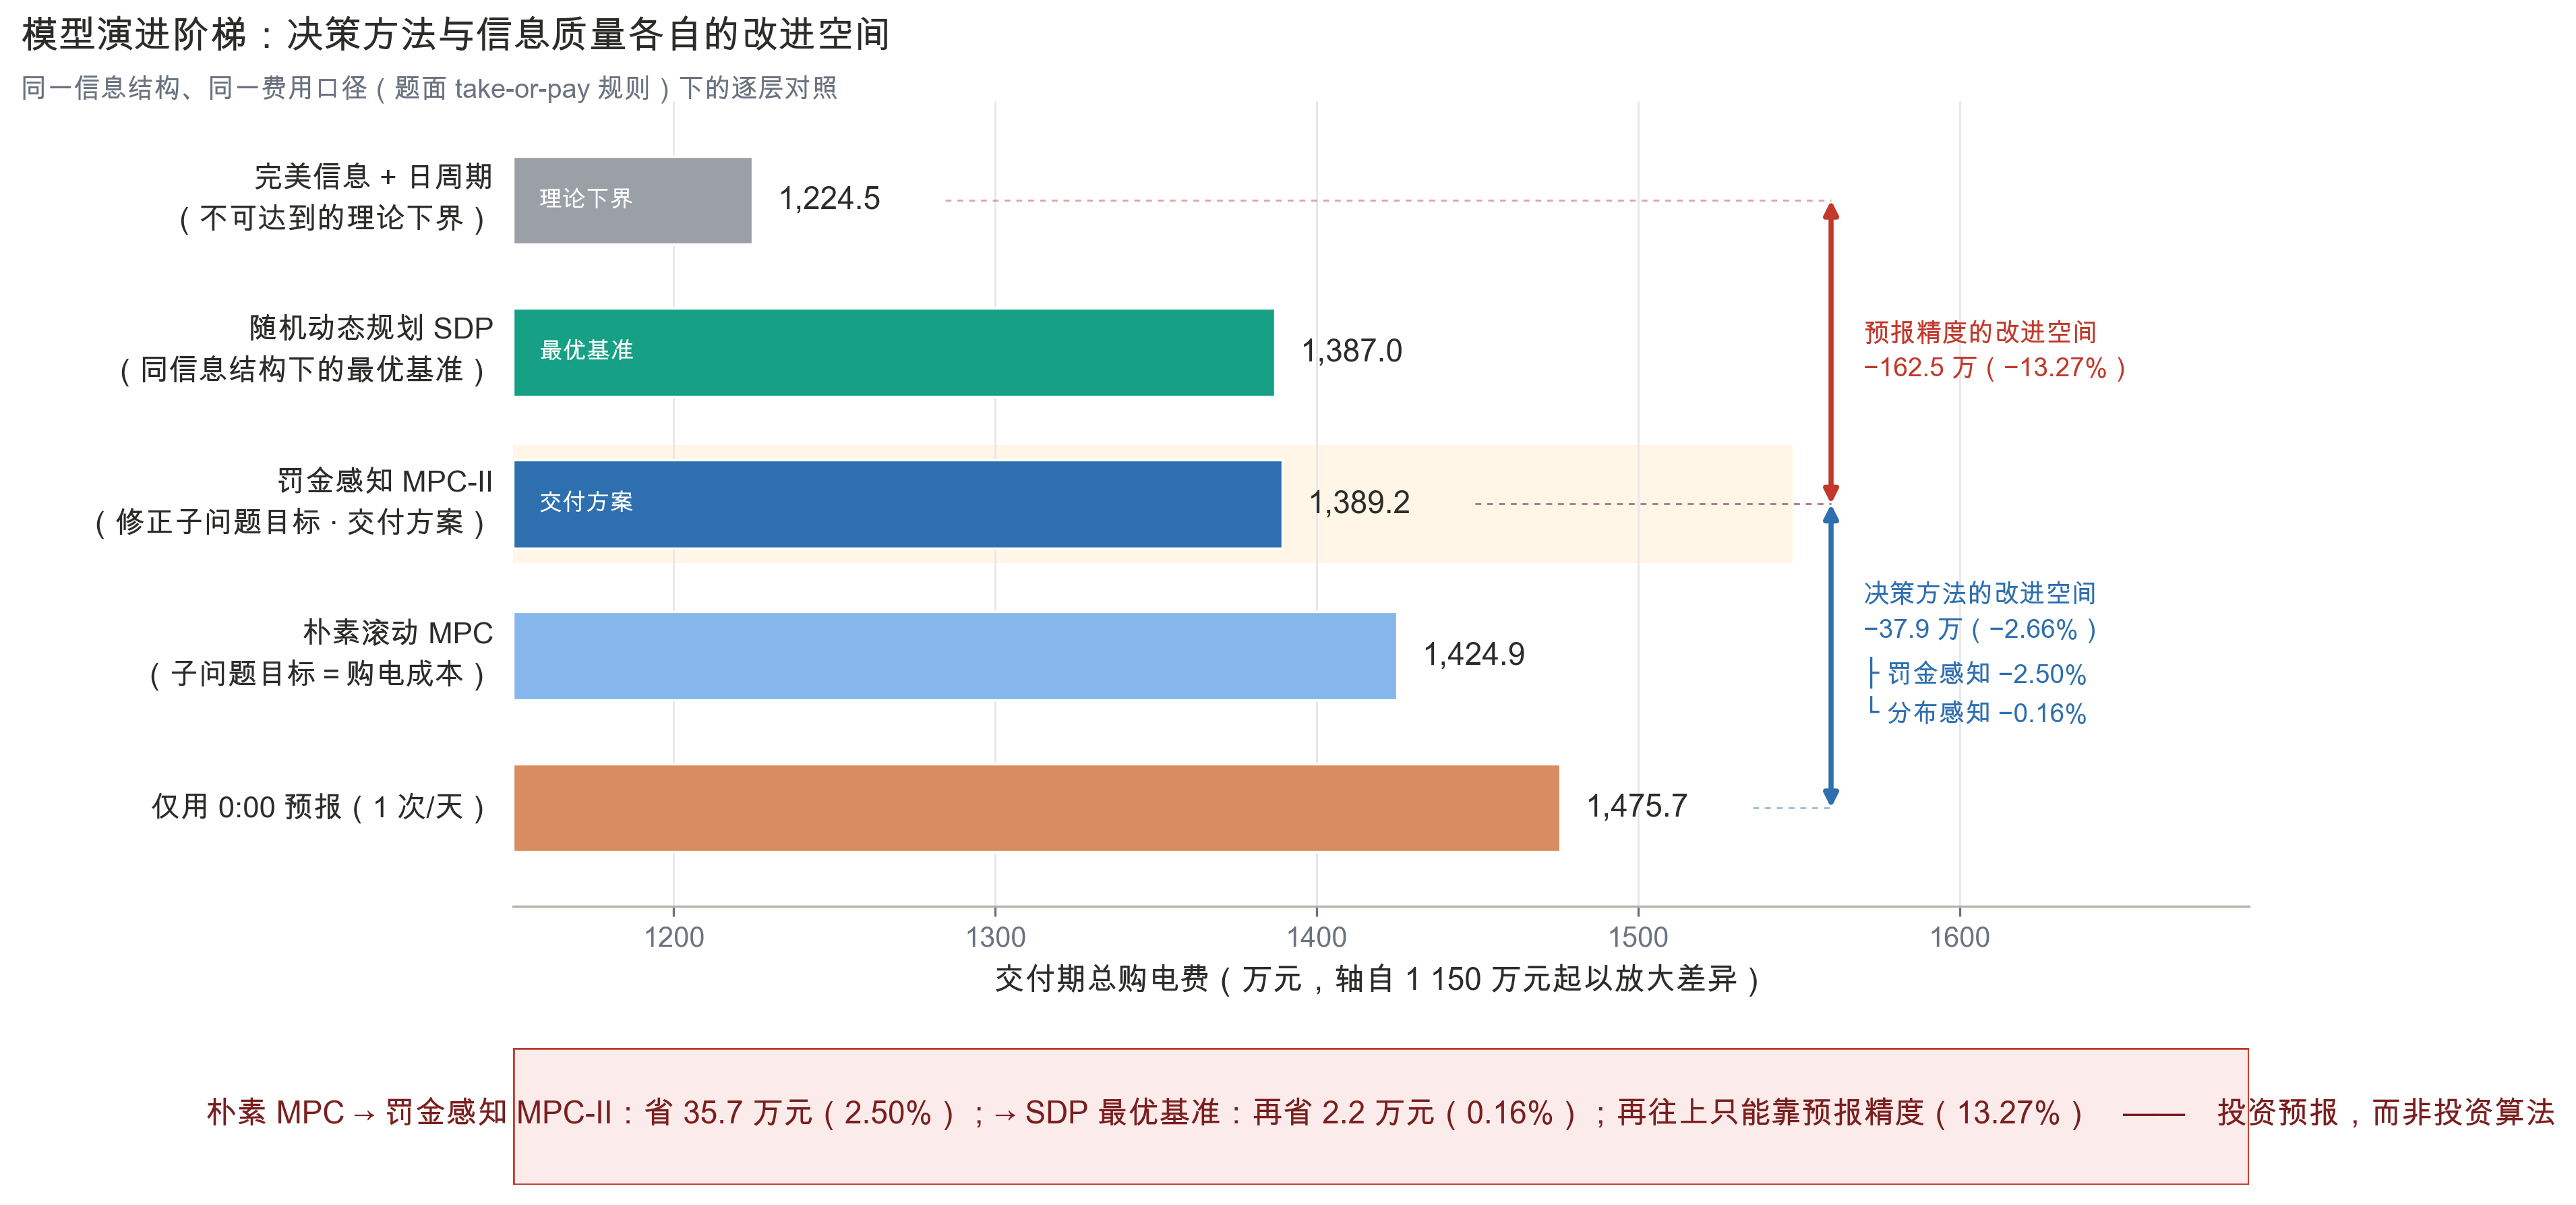
\includegraphics[width=0.98\textwidth]{fig_model_ladder.png}
\caption{模型演进阶梯：五方案费用对比与两类改进空间的分离量化}\label{fig:ladder}
\end{figure}

\section{风险与鲁棒性分析}\label{sec:risk}

\subsection{场景法：尾部风险极小}
以\textbf{整日分块自举}生成 50 组全年场景（保留预报误差的日内相关——逐时段独立重采样会人为抹平它并使费用低估 4.8\%；同时施加夜间掩码防止把黄昏残差注入\textbf{实际应为 0}的深夜时段）。生成器以\textbf{实测光伏 + 实测预报重跑}校验，分毫不差复现基准值。结果：场景期望 1\,452.2 万元（基准 $+1.92\%$），标准差 4.2 万元，$\VaR_{95}=1\,457.6$ 万，$\CVaR_{95}=1\,458.3$ 万元（\textbf{超期望仅 0.42\%}）——储能 + 滚动调整机制\textbf{自带强风险平滑能力}（图~\ref{fig:risk}）。

\subsection{鲁棒对等：$\Gamma$ 型预算不确定集}
对每个时段按 $\Gamma\cdot\sigma(k)$ 对预报保守打折（Bertsimas--Sim 型，鲁棒对等仍为 LP 同阶规模）。$\Gamma$ 扫描呈\textbf{非单调}：$\Gamma\approx0.25$ 时期望与 $\CVaR_{95}$ \textbf{同时}最低（白天预报本身略偏保守，适度保守化即隐式偏差修正）；$\Gamma>0.5$ 后进入经典\textbf{期望换最坏}权衡。

\subsection{电价情景：水平效应才是一阶驱动}
经验 5/95 分位电价情景下，交付期总费用为 1\,017.8 / 1\,486.0 / 1\,765.5 万元——电价风险区间 747.7 万元（50.3\%），远大于预报尾部风险两个量级内的贡献：\textbf{电价的系统性水平（而非其逐时波动）才是费用的一阶驱动因素}。

\begin{figure}[H]\centering
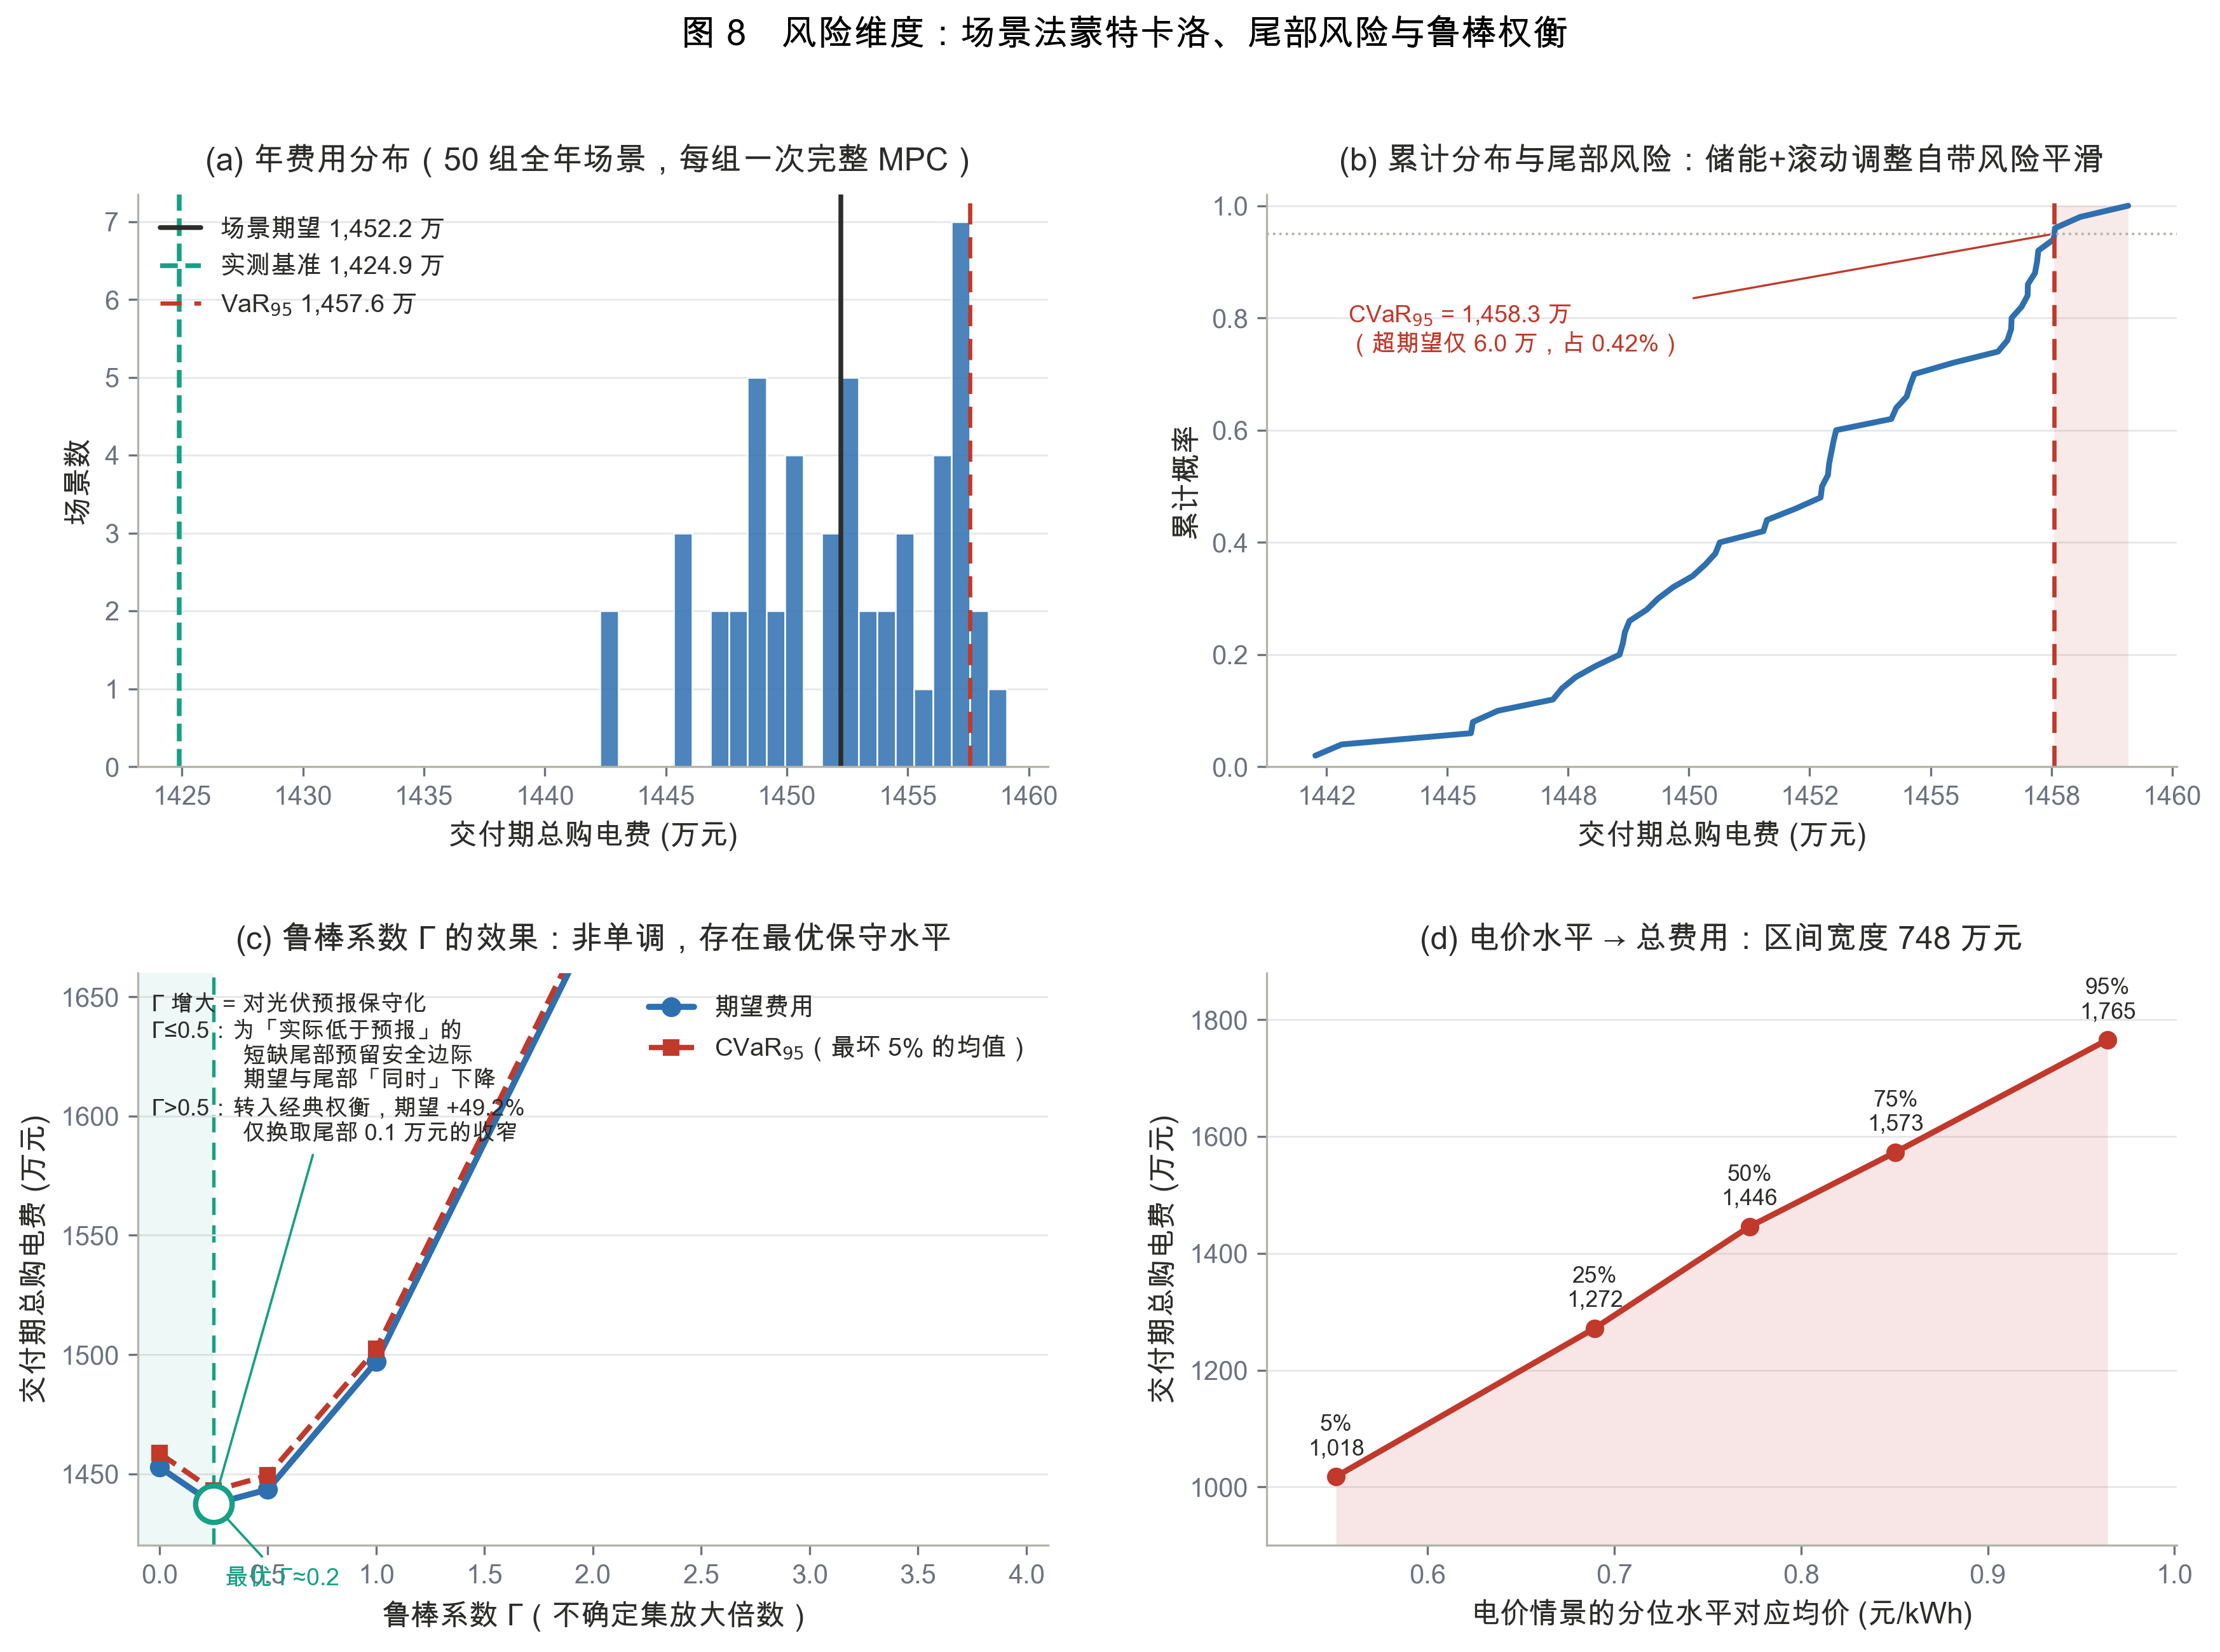
\includegraphics[width=0.98\textwidth]{fig_risk.png}
\caption{风险分析：(a) 50 场景费用分布与 CVaR；(b) VaR/CVaR 收敛；(c) 鲁棒系数 $\Gamma$ 的非单调效应；(d) 电价情景区间}\label{fig:risk}
\end{figure}

\section{灵敏度分析与模型检验}\label{sec:check}

\subsection{灵敏度}
对 $\eta\in[0.80,0.95]$、$P_{\max}\in[2500,7500]$、预报误差放大系数与六情景费用做扫描（图~\ref{fig:sens}）。要点：① 效率是高杠杆参数——$\eta$ 每降 0.01，全年费用上升约 0.8\%，且套利阈值 $1/\eta^2$ 相应上移；② $P_{\max}\ge5000$ 后费用几乎不再下降（储能功率已非瓶颈，容量才是），说明题目给定参数已近饱和；③ 六情景对比再次印证\textbf{预报误差 $\gg$ 电价波动}。

\begin{figure}[H]\centering
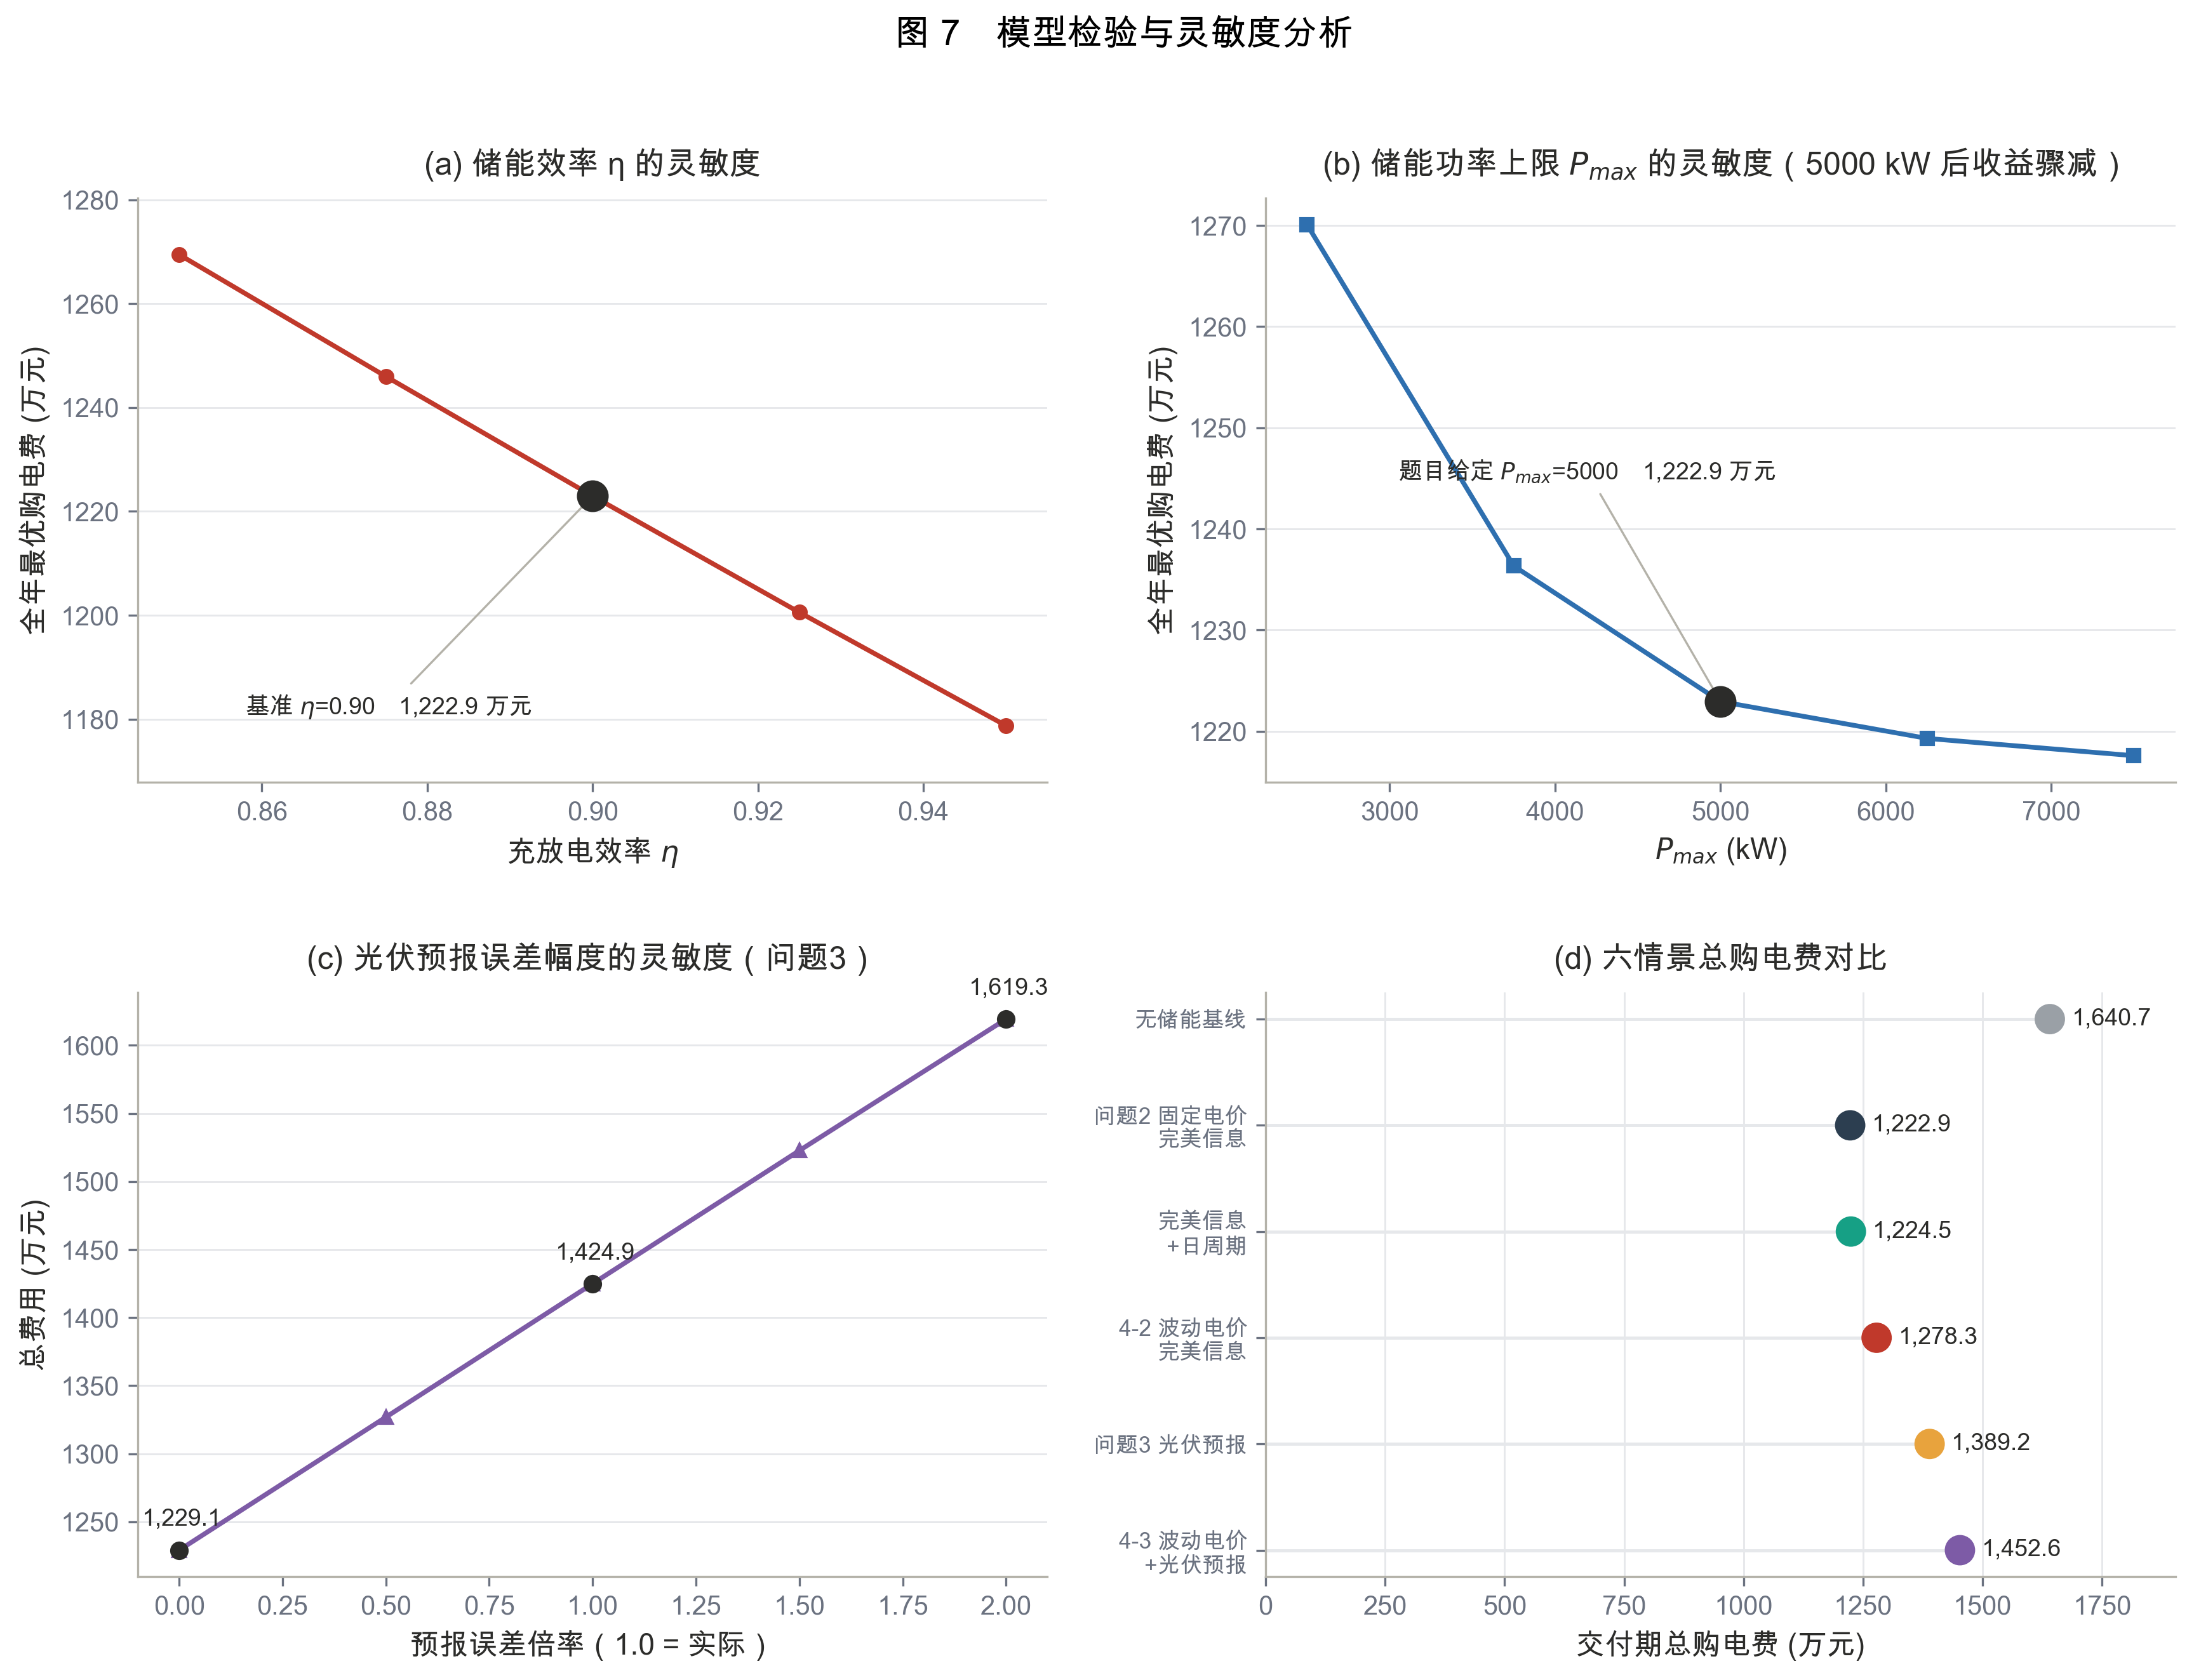
\includegraphics[width=0.98\textwidth]{fig_sensitivity.png}
\caption{灵敏度分析：(a) 效率 $\eta$；(b) 功率上限 $P_{\max}$；(c) 预报误差放大；(d) 六情景对比}\label{fig:sens}
\end{figure}

\subsection{模型检验（8 项）}
\begin{enumerate}[label=\textbf{T\arabic*.}]
  \item LP 解的自检：功率平衡与储能动态残差 $>10^{-4}$ 即中止（曾在调试中捕获约束矩阵列错位导致的\textbf{凭空造电}）；
  \item 理论下界校验：问题1 购电量 59\,482.7 kWh $\ge$ 净负荷下界 56\,729 kWh，差值全部为效率损耗；
  \item 互补松弛：购电时段 $\mu_t=c_t$，残差 $1.1\times10^{-16}$；
  \item 售电禁令：全部解中 $v_t\le\max(L_t-S_t,0)$ 无一违反；
  \item 场景生成器校验：以实测输入重跑，精确复现基准费用；年发电量偏差 $-0.58\%$；
  \item 预报对齐校验：跨日预报按 $(6h_0)$ 移位对齐，逐检查点子问题残差 $<10^{-9}$；
  \item SDP 校验：值函数单调、终端约束生效、策略查表残差可忽略；
  \item 交付文件校验：五份 result 文件逐格与官方模板核对行列标签与单位（kWh）。
\end{enumerate}

\section{模型评价与推广}

\textbf{优点}：① 四问同源、信息集递进，模型体系自洽统一；② 从题面 take-or-pay 条款推出\textbf{调整环节边际成本是罚金}，修正子问题目标即省 2.50\%——建模细节直接转化为经济效益；③ SDP 基准使\textbf{逼近最优}成为有参照的量化命题（差 0.16\%）；④ 全部结论由 8 项检验、6 组灵敏度、50 场景风险度量与鲁棒双视角支撑。

\textbf{缺点与改进}：① SDP 动作仍为 250 kW 离散（细化收益不抵风险）；② 预报误差库按分箱拟合，样本外漂移需在线更新；③ 鲁棒集为静态 box，可推广为数据驱动的 Wasserstein 球；④ 储能模型未计入老化成本，扩展时可引入循环寿命折损项进入目标函数。

\textbf{推广}：本文\textbf{信息集递进 + 罚金感知滚动 + 最优性基准}的三层范式，可直接迁移至库存管理（take-or-pay 合同）、云计算竞价实例与电动车充电调度等\textbf{承诺量 + 违约罚金 + 短缺惩罚}结构的问题。

\section*{AI 工具使用声明}
\addcontentsline{toc}{section}{AI 工具使用声明}
本团队在建模与论文撰写过程中使用了 AI 工具辅助：数据预处理与求解代码的调试、图表绘制脚本的编写、以及文字润色。所有模型建立、口径判断、结果核验与结论推导均由团队独立完成并逐项复核；AI 未参与任何核心创新点的提出。按照竞赛规定，AI 工具使用详情已单独整理并随支撑材料提交。

\section*{参考文献}
\addcontentsline{toc}{section}{参考文献}
\begin{enumerate}[label={[\arabic*]}]
  \item Mayne D Q, Rawlings J B, Rao C V, et al. Constrained model predictive control: Stability and optimality[J]. Automatica, 2000, 36(6): 789--814.
  \item Bertsimas D, Sim M. The price of robustness[J]. Operations Research, 2004, 52(1): 35--53.
  \item Bertsekas D P. Dynamic Programming and Optimal Control, Volume I[M]. 4th ed. Belmont: Athena Scientific, 2017.
  \item Powell W B. Approximate Dynamic Programming: Solving the Curses of Dimensionality[M]. 2nd ed. Hoboken: Wiley, 2011.
  \item Rockafellar R T, Uryasev S. Optimization of conditional value-at-risk[J]. Journal of Risk, 2000, 2: 21--42.
  \item Birge J R, Louveaux F. Introduction to Stochastic Programming[M]. 2nd ed. New York: Springer, 2011.
  \item 姜启源, 谢金星, 叶俊. 数学模型[M]. 第5版. 北京: 高等教育出版社, 2018.
  \item 司守奎, 孙兆亮. 数学建模算法与应用[M]. 第2版. 北京: 国防工业出版社, 2015.
  \item Huang Q, et al. HiGHS: High-performance linear and mixed integer solvers[J]. Mathematical Programming Computation, 2023, 15: 587--603.
\end{enumerate}

\newpage
\appendix
\section{附录A：支撑材料与代码清单}
\begin{table}[H]\centering\small
\caption{代码模块与功能（全部源码随支撑材料提交，可一键复现）}
\begin{tabular}{ll}
\toprule
模块 & 功能\\
\midrule
cumcm\_core.py & 数据加载、预报降尺度与跨日对齐、LP 求解器（含解自检）\\
cumcm\_pen.py & 罚金感知 LP 子问题（MPC-II 核心，式 \eqref{eq:penobj}）\\
cumcm\_write.py & 官方模板填充写出（result1--4-3.xlsx）\\
04\_p1 / 05\_p2.py & 问题1、2 求解\\
06\_p3 / 07\_p4.py & 问题3、4 滚动仿真与交付文件生成\\
12\_risk / 14\_robust.py & 50 场景风险度量、$\Gamma$ 型鲁棒对等\\
18\_sdp.py & 随机动态规划基准（97$\times$41 网格，30 s）\\
09/10/11/13/15/16/21\_*.py & 论文全部插图的生成脚本\\
\bottomrule
\end{tabular}
\end{table}

支撑材料另含：result1--result4-3.xlsx（官方模板格式）、全部中间结果 npz/csv、AI 工具使用详情。

\section{附录B：口径与单位说明}
\begin{itemize}
  \item 表中购电量、充放电量单位均为 kWh；功率为 kW；费用为元；
  \item 问题3/4 的\textbf{购电量}列给出\textbf{调整后执行量}（即实际交付量）；计划购电量见支撑材料 result3/result4-3 的\textbf{计划购电量}工作表；
  \item 问题1 全天 144 时段、问题2--4 交付期 334 天（2025-02-01 至 12-31）；
  \item 口径A（主口径）：计划量全额计费；调整不足按 0.5 倍、超出按 1.5 倍计罚金；短缺按 5 倍紧急购电。
\end{itemize}

\end{document}
